\documentclass[10pt,a4paper]{article}
\usepackage{sbc-template}
\usepackage{amsmath}
\usepackage{amsfonts}
\usepackage{amssymb}
\usepackage{graphicx}
\usepackage{setspace}
\usepackage{tensor}
\usepackage{listings}
\usepackage{float}
\usepackage{subcaption}
\usepackage{multirow}
\usepackage[table,xcdraw]{xcolor}
\usepackage[algoruled, linesnumbered, portuguese]{algorithm2e}
\usepackage{natbib}
\bibliographystyle{abbrvnat}
\lstset{
  language=C,
  basicstyle=\ttfamily\small,
  extendedchars=true,
  showspaces=false,
  showstringspaces=false,
  numbers=left,
  numberstyle=\tiny,
  breaklines=true
}
\usepackage{fancyhdr}
\rhead{\thepage}
\lhead{MP 2025 IF Goiano}
\chead{}
\lfoot{}
\cfoot{}
\rfoot{}
\pagestyle{fancy}
\setlength{\headheight}{15pt}
\everymath{\displaystyle}
\usepackage{multicol}
\setlength{\columnsep}{1cm}
\usepackage{vwcol}
\usepackage{caption}
\usepackage{tabularx}
\usepackage[hidelinks]{hyperref}
\usepackage{mdframed}
\usepackage{tcolorbox}
\usepackage{tikz}
\tcbuselibrary{skins}

\tcbuselibrary{listings,breakable}

\tcbset{
    listing only,
    breakable,
    enhanced,
    frame hidden,
    arc=0pt,
    outer arc=0pt,
    top=0pt,
    bottom=0pt,
    left=0pt,
    right=0pt,
    colback=white,
    fontupper=\ttfamily\footnotesize,
}

\begin{document}

\thispagestyle{empty}

\begin{figure}[! tbp]
    \centering
    \subfloat{
\includegraphics[width=0.35\textwidth]{fig/if rio verde.png}}
    \hfill
 \subfloat{
\includegraphics[width=0.45\textwidth]{fig/abobora.png}}
 \vspace{2 cm}
\end{figure}
\begin{center}
\huge \textbf{Biblioteca de algoritmos e códigos em C++ para consulta nas maratonas de programação}
\vspace{1 cm}

\Large Esta biblioteca foi criada para consulta dos principais algoritmos utilizados nas maratonas de programação, esses algoritmos  foram implementados utilizando a linguagem C++,visando:

\begin{enumerate}
    \item Auxiliar na aprendizagem de programação e suas aplicações;

     \item Desenvolver soluções eficientes para resolver problemas computacionais;

        \item Compreender algoritmos e suas técnicas;
        
         \item Incentivar a participação em maratonas;
         
    \item O trabalho tem como objetivo:
    
    \begin{enumerate}
        \item \textit{Motivar os alunos em competições}
        \item \textit{Criar um material impresso que possa ser utilizado:}
    \end{enumerate}
\end{enumerate}
\end{center}

\section{Complexidade}
\textbf{O que é a complexidade de um algoritmo?}

Complexidade de algoritmo refere-se à medida de eficiência de um algoritmo em termos de tempo e espaço. Ela avalia o quanto de recurso computacional (como CPU ou memória) que um algoritmo requer para resolver o problema conforme sua entrada cresce. A complexidade é geralmente expressa na notação Big O, que descreve o comportamento assintótico do algoritmo ao considerar o tamanho da entrada para um pior caso. Por exemplo, um algoritmo com complexidade O(n) tem um tempo de execução que cresce linearmente com o tamanho da entrada, enquanto um com complexidade $O(n^2)$ tem um tempo de execução com crescimento quadrático.

Existem dois tipos principais de complexidade: complexidade de tempo e complexidade de espaço. A complexidade de tempo se refere à quantidade de tempo que um algoritmo leva para processar uma entrada de tamanho n, enquanto a complexidade de espaço se refere à quantidade de memória necessária. Entender a complexidade ajuda na escolha de algoritmos mais eficientes, especialmente para grandes conjuntos de dados, permitindo soluções que equilibram entre rapidez e uso de recursos, fundamental para otimização em desenvolvimento de software e ciência da computação.

\subsection*{Notação $O$}
    Quando existe um limite assintótico superior, a notacão $O$,é utilizada. Para uma dada função g(n), denotamos por O((g(n)) (lê-se "Ó grande de g de n" ou, "ó de g de n") o conjunto de funções $O(g(n)) =f(n)$( existem constantes positivas $c$ e $n_0$ tais que $0\leq f(n) \leq c*g(n)$ para todo $ n \geq n_0$).
    
Usamos a notação $O$ para dar um limite superior a uma função, dentro de um fator constante. Para todos os valores $n$ em $n_0$ ou à direita de $n_0$, o valor da função $f(n)$ está abaixo de $c*g(n)$.

 Tendo em vista que a notação $O$ descreve um limite superior, quando a empregamos para limitar o tempo de execução do pior caso de um algoritmo temos um limite para o tempo de execução do algoritmo em cada entrada\cite{AlgoritmoCormen2009}.




\subsection{Complexidade O(1)}

A complexidade $O(1)$, ou complexidade de tempo constante, significa que um algoritmo leva o mesmo tempo para executar, independentemente do tamanho da entrada. Isso ocorre porque o algoritmo realiza um número fixo de operações, como calcular a distância entre dois pontos ou acessar um elemento específico em matrizes.

A fim de  demonstrar o sistema de complexidade $O(1)$ será utilizado um exemplo como base, neste exercício  é necessário criar um programa que quantifique diferentes tipos de pisos para uma sala qualquer, onde não basta apenas ter área da sala, pois os pisos se diferem entre inteiros e cortados, então leva-se em consideração os espaços não completos do chão da sala.

A complexidade $O(1)$, trabalha com uma constante durante todo o seu processo, para fins de contagem a constante é desprezada.
Segue o exemplo:
\newpage
\begin{center}
Piso da escola

{ OBI 2018}

Timelimit: $1$	
\end{center}

 O colégio pretende trocar o piso de uma sala de aula e a diretora aproveitou a oportunidade para passar uma tarefa aos alunos. A sala tem o formato de um retângulo de largura $L$ metros e comprimento $C$ metros, onde $L$ e $C$ são números inteiros. A diretora precisa comprar lajotas de cerâmica para cobrir todo o piso da sala. Seria fácil calcular quantas lajotas seriam necessárias se cada lajota fosse um quadrado de $1$ metro de lado. O problema é que a lajota que a diretora quer comprar é um quadrado que possui $1$ metro de diagonal, não de lado. Além disso, ela quer preencher o piso da sala com as diagonais das lajotas alinhadas aos lados da sala, como na figura.

A loja vai fornecer lajotas do tipo $1$: inteiras; do tipo $2$, que correspondem à metade das do tipo $1$, cortadas ao longo da diagonal; e lajotas do tipo $3$, que correspondem à metade do tipo $2$. Veja os três tipos de lajotas na figura.


\includegraphics[width=1.0\textwidth]{fig/Piso da Escola.png}
 Está muito claro que sempre serão necessárias $4$ lajotas do tipo $3$ para os cantos da sala. A tarefa que a diretora passou para os alunos é calcular o número de lajotas dos tipos $1$ e $2$ que serão necessárias. Na figura, para $L=3$ e $C=5$, foram necessárias $23$ do tipo $1$ e $12$ do tipo $2$.

Seu programa precisa computar, dados os valores de $L$ e $C$, a quantidade de lajotas do tipo $1$ e do tipo $2$ necessárias.

\vspace{0.3cm}
\textbf{Entrada}

A entrada consiste de um único número inteiro $L$ indicando a largura da sala. A segunda linha contém um inteiro $C$ representando o comprimento da sala, conforme dados da tabela~\ref{tabela01}. 

\vspace{0.3cm}
\textbf{Saída}

Imprima duas linhas na saída. A primeira deve conter um inteiro, representando o número de lajotas do tipo $1$ necessárias. A segunda deve conter um inteiro, indicando o número de lajotas do tipo $2$.

\textbf{Restrições}
\begin{itemize}
    \item $1 \leq L,C \leq 100$
\end{itemize}

\begin{table}[!ht]
    \centering
    \begin{tabular}{|p{7cm}|p{7cm}|}
        \hline
        \begin{center}
            \vspace{-0.3cm}
            \textbf{Exemplos de Entrada}
            \vspace{-0.3cm}
        \end{center} 
         &  
        \begin{center}
            \vspace{-0.3cm}
            \textbf{Exemplos de Saída}
            \vspace{-0.3cm}
        \end{center} \\ \hline
         \texttt{3} & \texttt{23} \\
         \texttt{5} & \texttt{12} \\
         \hline
         \texttt{1} & \texttt{1} \\
         \texttt{1} & \texttt{0}\\
         \hline
    \end{tabular}
    \caption{Exemplos de entradas e saídas}
    \label{tabela01}
\end{table}

%---------------------------------------------


\begin{table}[ht]
\centering

\label{tab:algoritmo1}
\begin{tabular}{|p{8cm}|c|c|}
\hline
\textbf{\cellcolor[HTML]{C0C0C0}Algoritmo} & \textbf{\cellcolor[HTML]{C0C0C0}Custo} & \textbf{\cellcolor[HTML]{C0C0C0}Complexidade} \\
\hline
\begin{minipage}{8cm}
{
        \begin{algorithm}[H]
            \caption{Piso da Sala}
            \label{alg:01}
            \SetAlgoLined
          \small  \Inicio{
            \textit{Declare} $L, C, T1, T2$ \textit{inteiro} \\
                \textit{Leia} $T1, T2$ \\
                $T1 \leftarrow L * C + ( L - 1) * ( C - 1)$ \\
                $T2 \leftarrow ( L - 1) * 2 + ( C - 1) * 2$ \\
                \textit{Escreva} $T1$ \\
                \textit{Escreva} $T2$ \\
                }
        \end{algorithm}}
\end{minipage} 
& 
\begin{minipage}{2cm}

C1 \\
C2\\
C3 \\
C4 \\
C5 \\
C6 \\
C7 \\
C8 \\
K\\
\end{minipage}
&
\begin{minipage}{2cm}

O(1) \\
O(1) \\
O(1) \\
O(1) \\
O(1)\\
O(1)\\
O(1) \\
O(1) \\
O(1)\\

\end{minipage}
\\
\hline
\end{tabular}
\end{table}


\begin{equation}
T(n)=({C_1}*1)+({C_2}*1)+({C_3}*1)+({C_4}*1)+({C_5}*1)+({C_6}*1)+({C_7}*1)+({C_8}*1)
\end{equation}

\begin{equation}T(n)=({C_1}+{C_2}+{C_3}+{C_4}+{C_5}+{C_6}+{C_7}+{C_8})*1\end{equation}
\begin{equation}\textit{Considere K} = {C_1}+{C_2}+{C_3}+{C_4}+{C_5}+{C_6}+{C_7}+{C_8}\end{equation}

\begin{equation}
    T(n)= K*1 = O(1)
\end{equation}
\begin{center}
\begin{minipage}{0.5\textwidth}
    \lstinputlisting[language=C++]{code/piso1.cpp}
\end{minipage}
\end{center}
\newpage

\subsection{Complexidade O(n)}
Uma complexidade $O(n)$ (complexidade linear) significa que o tempo ou espaço necessário para executar um algoritmo aumenta de forma linear com o tamanho da entrada. Em outras palavras, se você dobrar o tamanho da entrada, o algoritmo também dobrará em tempo de execução ou espaço de memória.

Para demonstrar a complexidade $O(n)$ um exercício retirado do site~\cite{beecrowd1} de busca em um vetor foi escolhido, a atividade em questão consiste em procurar dentro de uma lista de números qual é o menor valor entre eles, destacando também a sua posição dentro da lista.

\begin{center}
\large Menor e Posição

{ BeeCrowd 1180}

Timelimit: $1$	
\end{center}

Faça um programa que leia um valor $N$. Este $N$ será o tamanho de um vetor $X[N]$. A seguir, leia cada um dos valores de X, encontre o menor elemento deste vetor e a sua posição dentro do vetor, mostrando esta informação.

\vspace{0.3cm}
\textbf{Entrada}

A primeira linha de entrada contém um único inteiro $N (1 < N < 1000)$, indicando o número de elementos que deverão ser lidos em seguida para o vetor $X[N]$ de inteiros. A segunda linha contém cada um dos $N$ valores, separados por um espaço. Vale lembrar que nenhuma entrada haverá números repetidos.

\vspace{0.3cm}
\textbf{Saída}
A primeira linha apresenta a mensagem “Menor valor:” seguida de um espaço e do menor valor lido na entrada. A segunda linha apresenta a mensagem “Posição:” seguido de um espaço e da posição do vetor na qual se encontra o menor valor lido, lembrando que o vetor inicia na posição zero.

\begin{table}[!ht]
    \centering
    \begin{tabular}{|p{7cm}|p{7cm}|}
        \hline
        \begin{center}
            \vspace{-0.3cm}
            \textbf{Exemplos de Entrada}
            \vspace{-0.3cm}
        \end{center} 
         &  
        \begin{center}
            \vspace{-0.3cm}
            \textbf{Exemplos de Saída}
            \vspace{-0.3cm}
        \end{center} \\ \hline
         \texttt{10} & \texttt{Menor valor: -5} \\
         \hline
         \texttt{1,2,3,4,-5,6,7,8,9,10} & \texttt{Posicao: 4} \\
         \hline
    \end{tabular}
    \caption{Exemplos de entradas e saídas}
    \label{tabela02}
\end{table}



\begin{table}[ht]
\centering
\caption{Exemplos de entradas e saídas}
\label{tab:algoritmo2}
\begin{tabular}{|p{8cm}|c|c|}
\hline
\textbf{\cellcolor[HTML]{C0C0C0}Algoritmo} & \textbf{\cellcolor[HTML]{C0C0C0}Custo} & \textbf{\cellcolor[HTML]{C0C0C0}Complexidade} \\
\hline
\begin{minipage}{8cm}
\begin{algorithm}[H]
 \caption{Menor e Posicao}
\SetAlgoLined
Declare $X, N, M, POS$ inteiro\;
Leia $N$\;
\For{$X \leftarrow 0$ \textbf{até} $N-1$ faça}{
    Leia $P[X]$\;
}
$M \leftarrow 0$\;
\For{$X \leftarrow 1$ \textbf{até} $N-1$ faça}{
    \If{$P[X] < P[M]$}{
        $M \leftarrow X$\;
    }
}
Escreva $P[M]$\;
Escreva $M$\;
\end{algorithm}
\end{minipage} 
& 
\begin{minipage}{2cm}
C1 \\
C2\\
C3 \\
C4 \\
C5 \\
C6 \\
C7 \\
C8 \\
C9 \\
    C10 \\
C11 \\
C12 \\
C13
\end{minipage}
&
\begin{minipage}{2cm}
1 \\
1 \\
1 \\
1 \\
$n$ \\
$n$ \\
1 \\
$n-1$ \\
$n-1$ \\
$n-1$ \\
$n-1$ \\
1 \\
1
\end{minipage}
\\
\hline
\end{tabular}
\end{table}


\begin{equation}
T(n) = C_1*1 + C_2*1 + C_3*1 + C_4*(n+1) + C_5*n + C_6*1+ C_7*1 + C_8*n
\end{equation}
\begin{equation}
+ C_9*(n-1) + C_10*(n-1) + C_11*1 + C_12*1 + C_13*1 +  C_14*1 + C_15*1
\end{equation}
\begin{equation}
    T(n)= K*(1 + 1 + 1 + n+1 + n + n + 1 + n + n-1 + n-1 + n-1 + n-1 + 1 + 1 + 1)
    \end{equation}
    \begin{equation}
    T(n)= 8*n + 4 =O(n)
    \end{equation}
\begin{center}
\begin{minipage}{0.5\textwidth}
    \lstinputlisting[language=C++]{code/resol++.cpp}
\end{minipage}
\end{center}


    
    \newpage



\subsection{Complexidade O(n²)}

A complexidade O(n²) é uma medida de desempenho de algoritmos que indica que o tempo de execução cresce quadraticamente com o tamanho da entrada, representado por $'n'$. Isso significa que, se o tamanho da entrada dobrar, o tempo de execução será aproximadamente quatro vezes maior, devido ao fator quadrático. Algoritmos com essa complexidade frequentemente envolvem dois loops aninhados, onde cada elemento da entrada é comparado ou processado em relação a todos os outros elementos.

Um exemplo clássico de algoritmo com complexidade O(n²) é o Bubble Sort, onde, para cada elemento de uma lista, são feitas comparações com os elementos subsequentes para realizar trocas e ordenar os dados. Em um caso médio ou pior, o algoritmo precisa percorrer a lista n vezes, e em cada iteração, realiza até n comparações ou operações, resultando em n * n = n² aoperações. Essa característica torna esses algoritmos ineficientes para grandes volumes de dados, pois o custo computacional aumenta rapidamente.

Embora algoritmos O(n²) sejam menos eficientes do que aqueles com complexidades lineares O(n) ou logarítmicas O(log n), eles ainda têm utilidade em cenários com entradas pequenas ou quando a simplicidade de implementação é mais importante que o desempenho. Além disso, podem servir como base para otimizações ou em situações específicas onde o pior caso raramente ocorre. No entanto, para aplicações de larga escala, é comum buscar alternativas mais eficientes, como algoritmos com complexidade O(n log n), típicos de métodos de ordenação mais avançados como Quick Sort ou Merge Sort.

Segue o exemplo representativo da complexidade O(n²):
\begin{center}
Fibonacci em Vetor

{Beecrowd 1176}

Timelimit: $1$	
\end{center}

Faça um programa que leia um valor e apresente o número de Fibonacci correspondente a este valor lido. Lembre que os 2 primeiros elementos da série de Fibonacci são 0 e 1 e cada próximo termo é a soma dos 2 anteriores a ele. Todos os valores de Fibonacci calculados neste problema devem caber em um inteiro de 64 bits sem sinal.

\vspace{0.3cm}
\textbf{Entrada}

A primeira linha da entrada contém um inteiro T, indicando o número de casos de teste. Cada caso de teste contém um único inteiro N $(0 \leq N \leq 60)$, correspondente ao N-esimo termo da série de Fibonacci.

\vspace{0.3cm}
\textbf{Saída}

Para cada caso de teste da entrada, imprima a mensagem "Fib(N) = X", onde X é o N-ésimo termo da série de Fibonacci.

%---------------------------------------------------------

\begin{table}[!ht]
    \centering
    \begin{tabular}{|p{7cm}|p{7cm}|}
        \hline
        \begin{center}
            \vspace{-0.3cm}
            \textbf{Exemplos de Entrada}
            \vspace{-0.3cm}
        \end{center} 
         &  
        \begin{center}
            \vspace{-0.3cm}
            \textbf{Exemplos de Saída}
            \vspace{-0.3cm}
        \end{center} \\ \hline
         \texttt{3} & \texttt{FIB(0) = 0} \\
         \texttt{0} & \texttt{FIB(4) = 3} \\
         \texttt{4} & \texttt{FIB(2) = 1} \\
         \texttt{2} & \texttt{}\\
         \hline
    \end{tabular}
    \caption{Exemplos de entradas e saídas}
    \label{tabela04}
\end{table}
%------------------------------------


\begin{center}
\begin{minipage}{0.5\textwidth}
    \lstinputlisting[language=C++]{fig/fibo.cpp}
\end{minipage}
\end{center}
$T(n)=C1*1+C2*1+C3*1+C4*(59)+C5*T+C6*T$\\
$T(n)=K+(C5+C6)*T$\\
$T(n)=a*T+b=O(T)$

\input{FundamentoAnálise/EA}
\input{FundamentoAnálise/ED}


\section{Abóbora Contest}
Como meio didático e objeto de estudos sobre as maratonas de programação, serão utilizadas as questões da maratona do Abóbora Contest (Maratona própria do Instituto Federal Goiano Campus Rio Verde). Nesta seção serão apresentadas as questões presentes nas provas dos anos de 2022,2023,2024 e 2025. Incluindo, também, suas respectivas soluções. 

\begin{center}
 {\large {\textbf 
{\large \textbf{Informações Gerais}}
}}
\end{center}

Cada caderno contém $10$ problemas exclusivos criados por professores e alunos do Instituto Federal Goiano - Campus Rio Verde.

Segue abaixo as regras da respectiva maratona:

\begin{enumerate}
    \item \textbf{Sobre os nomes dos programas}
    \begin{enumerate}
        \item Para soluções em C/C++ e Python 3.8, o nome do arquivo-fonte não é significativo, pode ser qualquer nome desde que tenha as extensões .c, .cc, .py3.
        \item Para linguagem Java sua solução deve ser chamado de codigo\_do\_problema.java, onde codigo\_do\_problema é a letra maiúscula que identifica o problema. Lembre que em Java o nome da classe principal deve ser igual ao nome do arquivo.
    \end{enumerate}
    \item \textbf{Sobre a entrada}
    \begin{enumerate}
        \item A entrada de seu programa deve ser lida da entrada padrão.
        \item A entrada é composta de um único caso de teste, descrito em um número de linhas que depende do problema.
        \item Quando uma linha da entrada contém vários valores, estes são separados por um único espaço em branco; a entrada não contém nenhum outro espaço em branco.
        \item Cada linha, incluindo a última, contém exatamente um caractere final-de-linha.
        \item O final da entrada coincide com o final do arquivo.
    \end{enumerate}
    \item \textbf{Sobre a saída}
    \begin{enumerate}
        \item A saída de seu programa deve ser escrita na saída padrão.
        \item Quando uma linha da saída contém vários valores, estes devem ser separados por um único espaço em branco; a saída não deve conter nenhum outro espaço em branco.
        \item Cada linha, incluindo a última, deve conter exatamente um caractere final-de-linha.
    \end{enumerate}
\end{enumerate}

\newpage

%\include{Problema/abóbora22}

\newpage

%\include{ProblemaB_H/ProblemaB}

\newpage

%\include{ProblemaC_MB/ProblemaC}

\newpage

%\include{ProblemaD_AJ/ProblemaD}

\newpage

%\include{ProblemaE_DC/ProblemaE}

\newpage

%\include{ProblemaF_A/ProblemaF}

\newpage

%\include{ProblemaG_MB/ProblemaG}

\newpage

%\include{ProblemaH_H/ProblemaH}

\newpage

%\include{ProblemaI_AJ/ProblemaI}

\newpage

%\include{ProblemaJ_U/ProblemaJ}

\newpage


\begin{center}
{{Maratona de Programação Abóbora Contest 2022}}

Problema A

Marlus e a Fila 

{\tiny by André}

Timelimit: $1$	
\end{center}			

Marlus é um coordenador de curso muito dedicado do curso de computação do NuCAT. Os alunos estão enfrentando um grande problema na entrada do NuCAT, todos querem entrar no mesmo horário gerando assim um grande tumulto. Marlus reuniu com os cavalheiro do NDE para tentar resolver o problema. Depois de muita discussão o NDE resolveu ordenar os alunos pelo número de matricula, e organizando a entrada pela ordem crescente. Mas Marlus precisa de sua ajuda para desenvolver o programa pois ele está muito ocupado com seu novo doutorado.

\vspace{0.3cm}
\textbf{Entrada}
Para cada dia será lido um inteiro $N$, $1 \leq  N  \leq  10^{4}$, que representa o número de alunos disponíveis na entrada. Depois será lido os $N$ números de matriculas.

\vspace{0.3cm}
\textbf{Saída}
Para cada dia, imprimir os  número de  matriculas ordenados em ordem crescente.

\begin{table}[h]
    \centering
    \begin{tabular}{|p{7cm}|p{7cm}|}
        \hline
        \begin{center}
            \vspace{-0.3cm}
            \textbf{Exemplos de Entrada}
            \vspace{-0.3cm}
        \end{center} 
         &  
        \begin{center}
            \vspace{-0.3cm}
            \textbf{Exemplos de Saída}
            \vspace{-0.3cm}
        \end{center} \\ \hline
         \texttt{5} & \texttt{1 2 3 4 5} \\  
         \texttt{5 4 3 2 1} & \texttt{} \\
         \hline
    \end{tabular}
    \caption{Exemplos de entradas e saídas}
    \label{tab:inputI}
\end{table}

\newpage

\begin{center}
\noindent
\lstinputlisting{abobora_22/A/A22.cpp}
\end{center}
\begin{center}
Problema B

O Desafio do Chocolate do Zé do Grafo

{\small Nome do arquivo: B.c, B.cpp, B.java, ou B.py}

{\large Timelimit: $1$}

{\tiny Por André da Cunha Ribeiro}

\end{center}					

Todo competidor de maratona de programação sabe que as longas horas de um concurso exigem um combustível especial para o cérebro. E qual é o lanche preferido de 10 entre 10 programadores para manter o foco e a energia? Chocolate, é claro! A combinação de açúcar e cafeína parece ter sido feita sob medida para transformar um bug teimoso em um cobiçado "Accepted".

%Zé do Grafo, mais do que um professor, é um mentor que entende perfeitamente a rotina de seus alunos. Vendo sua equipe exausta após um treino intenso para a grande final da competição, ele aparece com o suprimento de energia definitivo: uma enorme barra de chocolate retangular, com N fileiras e M colunas.

%Mas, fiel ao seu estilo, Zé do Grafo não perderia a chance de um bom desafio. Ele colocou a barra de chocolate sobre a mesa e continuou: "O processo para dividir nosso prêmio é simples. A cada movimento, só podemos pegar um único pedaço de chocolate e quebrá-lo uma única vez, sempre em linha reta, seguindo um dos sulcos que dividem os quadrados. Cada quebra transforma um pedaço em dois. Vamos repetir isso até que toda a barra se transforme nos pequenos quadrados individuais de 1x1."

%Ele fez uma pausa e olhou para a equipe com um olhar astuto. "Agora, a pergunta que vale o primeiro pedaço: qual o número exato de quebras necessárias para completar a tarefa?"


Zé do Grafo, um famoso professor de Teoria dos Grafos e um ávido criador de quebra-cabeças, propôs um desafio para seus alunos. Ele apresentou uma barra de chocolate retangular, dividida em pequenos quadrados por sulcos, formando uma grade de $N$ fileiras e $M$ colunas.

O desafio é o seguinte: para dividir a barra de chocolate em $(N * M)$ quadrados de chocolate individuais, os alunos só podem realizar um tipo de movimento. A cada passo, eles podem pegar um único pedaço de chocolate e quebrá-lo ao longo de um dos sulcos (seja na horizontal ou na vertical), resultando em dois pedaços menores.

Sua tarefa é criar um programa que ajude os alunos do Zé do Grafo a descobrir rapidamente o número total de quebras necessárias para transformar a barra inteira em quadrados individuais.

\vspace{0.3cm}
\textbf{Entrada}
A entrada contém  na primeira linha o valor $1 \leq X \leq 1000$ que representa o número dos casos de teste. Seguido de $X$ leituras dos valores de $N,M$ $(1 \leq N,M \leq 10^9)$ indicando as dimensões dos chocolates. 


\vspace{0.3cm}
\textbf{Saída}
Para cada caso de teste, o programa deve produzir uma linha na saída, contendo um único inteiro que representa o número total de quebras necessárias para dividir o chocolate daquele caso de teste.

{\tiny
\begin{table}[h]
    \centering
    \begin{tabular}{|p{7cm}|p{7cm}|}
        \hline
        \begin{center}
            \vspace{-0.3cm}
            \textbf{Exemplos de Entrada}
            \vspace{-0.3cm}
        \end{center} 
         &  
        \begin{center}
            \vspace{-0.3cm}
            \textbf{Exemplos de Saída}
            \vspace{-0.3cm}
        \end{center} \\ \hline
         \texttt{4} & \texttt{3} \\  
         \texttt{2 2} & \texttt{23} \\
         \texttt{4 6} & \texttt{55} \\
         \texttt{7 8} & \texttt{836} \\
         \texttt{27 31} & \texttt{} \\
        \hline
    \end{tabular}
    \caption{Exemplos de entradas e saídas}
\end{table}}

\newpage

\begin{center}
\noindent
\lstinputlisting{abobora_25/B/B5.cpp}
\end{center}

\begin{center}
Problema C

Otimização de Rotas de Coleta de Solo - Simple Smart Agro

{\small Nome do arquivo: C.c, C.cpp, C.java, ou C.py}

{\large Timelimit: $2$}

{\tiny Por Alexandre da Silva}

\end{center}	

\footnotesize
			
A Simple Smart Agro está desenvolvendo um sistema automatizado para coleta de amostras de solo em uma fazenda. O sistema precisa otimizar as rotas de coleta para maximizar a eficiência do processo. Existem $N$ pontos específicos onde amostras de solo devem ser coletadas. O veículo de coleta parte sempre do depósito localizado na origem $(0, 0)$ e deve retornar ao mesmo ponto após coletar todas as amostras. Devido às características do terreno e dos equipamentos, o veículo só pode se mover nas direções cardeais (norte, sul, leste, oeste) e sempre em linha reta entre dois pontos consecutivos da rota. A distância entre dois pontos $(x_1, y_1)$ e $(x_2, y_2)$ é calculada usando a distância Manhattan: $|x_1 - x_2| + |y_1 - y_2|$.

\subsection*{Entrada}

\begin{itemize}
    \item A primeira linha contém um inteiro $N$ $(1 \leq N \leq 10)$, representando o número de pontos de coleta;
    \item As próximas $N$ linhas contêm dois inteiros $x_i$ e $y_i$ $(-1000 \leq x_i, y_i \leq 1000)$, representando as coordenadas do $i$-ésimo ponto de coleta;
       \item Todos os pontos de coleta são distintos entre si;
    \item Nenhum ponto de coleta coincide com a origem $(0,0)$.
\end{itemize}

\subsection*{Saída}

\begin{itemize}
    \item Uma única linha contendo um inteiro: a menor distância total (distância Manhattan) necessária para visitar todos os pontos de coleta e retornar à origem.
\end{itemize}

\subsection*{Exemplos}

\begin{center}
\begin{tabular}{|p{6cm}|p{4cm}|}
\hline
\textbf{Exemplo de Entrada} & \textbf{Exemplo de Saída} \\
\hline
\texttt{3} & \texttt{26} \\
\texttt{2 3} & \\
\texttt{7 1} & \\
\texttt{5 6} & \\
\hline
\texttt{4} & \texttt{42} \\
\texttt{3 4} & \\
\texttt{8 2} & \\
\texttt{12 8} & \\
\texttt{6 10} & \\
\hline
\texttt{1} & \texttt{8} \\
\texttt{2 2} & \\
\hline
\end{tabular}
\end{center}

\subsection*{Explicação do Primeiro Exemplo}

Partindo da origem $(0,0)$, temos os pontos de coleta em $(2,3)$, $(7,1)$ e $(5,6)$.
Uma rota ótima seria:
$(0,0) \rightarrow (2,3) \rightarrow (5,6) \rightarrow (7,1) \rightarrow (0,0)$

Calculando as distâncias:
\begin{itemize}
    \item $(0,0)$ para $(2,3)$: $|2-0| + |3-0| = 2 + 3 = 5$
    \item $(2,3)$ para $(5,6)$: $|5-2| + |6-3| = 3 + 3 = 6$
    \item $(5,6)$ para $(7,1)$: $|7-5| + |1-6| = 2 + 5 = 7$
    \item $(7,1)$ para $(0,0)$: $|0-7| + |0-1| = 7 + 1 = 8$
\end{itemize}

Distância total: $5 + 6 + 7 + 8 = 26$


\newpage

\begin{center}
\noindent
\lstinputlisting{abobora_25/C/C5.cpp}
\end{center}
\begin{center}
Problema D

Agência de Espionagem

{\small Nome do arquivo: D.c, D.cpp, D.java, ou D.py}

{\large Timelimit: $1$}

{\tiny Por Athos José}


\end{center}

A Agência Nacional de Espionagem mantém em seus cofres uma coleção de símbolos secretos, representados por uma sequência de letras. Esses símbolos podem ser reorganizados em qualquer ordem, de forma a formar novas mensagens.

Agentes inimigos, porém, estão tentando criar mensagens escondidas dentro dessas reorganizações. Uma mensagem inimiga é considerada possível se puder aparecer como uma sequência contínua de caracteres de alguma permutação dos símbolos guardados no cofre.

Sua missão é, para cada mensagem inimiga recebida, determinar se ela pode ser formada a partir dos símbolos da Agência.

\vspace{0.3cm}
\textbf{Entrada}

A primeira linha contém um inteiro $N$ ($1 \leq N \leq 10^5$), o número de mensagens inimigas a serem analisadas, seguido de uma string $S$ ($1 \leq |S| \leq 10^5$) representando os símbolos secretos do cofre.

Cada uma das próximas $N$ linhas contém uma string $Q_i$ ($1 \leq |Q_i| \leq 10^5$), representando uma mensagem inimiga a ser verificada.

A soma dos comprimentos de todas as mensagens $Q_i$ não excede $10^9$.

Todas as strings são compostas apenas de letras minúsculas do alfabeto inglês (a-z).

\vspace{0.3cm}
\textbf{Saída}

Para cada mensagem $Q_i$ imprima uma linha contendo:
\begin{itemize}
    \item ``SIM'', se a mensagem pode ser formada como substring de alguma permutação de $S$.
    \item ``NAO'',caso contrário.
\end{itemize}

\begin{table}[h]
    \centering
    \begin{tabular}{|p{7cm}|p{7cm}|}
       \hline
        \begin{center}
            \vspace{-0.3cm}
            \textbf{Exemplos de Entrada}
            \vspace{-0.3cm}
        \end{center} 
         &  
        \begin{center}
            \vspace{-0.3cm}
            \textbf{Exemplos de Saída}
            \vspace{-0.3cm}
        \end{center} \\ \hline
         \texttt{3 abac} & \texttt{SIM} \\  
         \texttt{caa} & \texttt{NAO} \\
         \texttt{aaa} & \texttt{SIM} \\  
         \texttt{bac} & \\
         \hline
    \end{tabular}
    \caption{Exemplos de entradas e saídas}
    \label{tab:inputB}
\end{table}

\newpage

\begin{center}
\noindent
\lstinputlisting{abobora_25/D/D5.cpp}
\end{center}
\begin{center}
Problema E

Estória da Estônia

{\small Nome do arquivo: E.c, E.cpp, E.java, ou E.py}

{\large Timelimit: $1$}

{\tiny Por Márcio Belo}

\end{center}			

O professor Márcio Belo sempre gostou de charadas matemáticas. Um dia ele se deparou com uma estória, pra lá da Estônia. Dado um número primo ímpar $p$, sempre é possível um triângulo de lados inteiros $x$, $y$ e $z$, em ordem crescente de tamanho com as seguintes propriedades: 
\begin{itemize}
    \item A diferença da soma dos lados menores do triângulo pelo lado maior é igual ao primo $p$; 
    \item A diferença da soma das áreas dos quadrados de lados $x$ e $y$ e a área do quadrado de lado $z$ é igual ao primo $p$. 
\end{itemize}
Em matematiquês:

\vspace{3mm}
Dado um primo $p \geq 3$, sempre existem triplas $(x,y,z)$, com $x \leq y \leq z$ que satisfazem: 
\begin{align*}
    x + y - z & = p \\
    x^{2} + y^{2} - z^{2} & = p 
\end{align*}
Quem são essas triplas $(x,y,z)$? Você pode ajudar o professor?

\vspace{0.3cm}
\textbf{Entrada}
Cada entrada contém uma única linha com o número primo $p$, com $(3 \leq p < 2^{16})$. 

\vspace{0.3cm}
\textbf{Saída}
O sistema deve retornar todas as triplas $(x,y,z)$ em ordem crescente de $x$. Uma tripla por linha,  

\begin{table}[h]
    \centering
    \begin{tabular}{|p{7cm}|p{7cm}|}
        \hline
        \begin{center}
            \vspace{-0.3cm}
            \textbf{Exemplos de Entrada}
            \vspace{-0.3cm}
        \end{center} 
         &  
        \begin{center}
            \vspace{-0.3cm}
            \textbf{Exemplos de Saída}
            \vspace{-0.3cm}
        \end{center} \\ \hline
         \texttt{3} & \texttt{(4,6,7)} \\  
         \hline
         \texttt{5} & \texttt{(6, 15, 16)} \\ 
          & \texttt{(7, 10, 12)} \\ 
         \hline
         \texttt{13} & \texttt{(14, 91, 92)} \\
         & \texttt{(15, 52, 54)} \\
         & \texttt{(16, 39, 42)} \\
         & \texttt{(19, 26, 32)} \\ 
         \hline
         \texttt{65267} & \texttt{(65268,2129923278,2129923279)} \\ 
          & \texttt{(97900,130534,163167)} \\ 
         \hline
    \end{tabular}
    \caption{Exemplos de entradas e saídas}

\end{table}

\newpage
\begin{center}
\noindent
\lstinputlisting{abobora_25/E/E5.cpp}
\end{center}
\begin{center}
Problema F

Monitorando Pragas

{\small Nome do arquivo: F.c, F.cpp, F.java, ou F.py}

{\large Timelimit: $1$}

{\tiny Por Emanuel Silva Araujo}

\end{center}

\footnotesize

O agricultor Seu Jayme sofre constantemente com infestações de insetos em sua lavoura de soja. Para reduzir perdas e otimizar o manejo, ele procurou a EMBRAPII para desenvolver uma ferramenta de monitoramento diário de pragas.
Sua tarefa como programador é implementar um programa que leia os valores de população diária e identifique situações de risco, emitindo alertas de acordo com os seguintes critérios:
%Critérios de Alerta
    \begin{itemize}
        \item  Alerta por pico diário [Pico]
        \begin{itemize}
            \item Se em qualquer dia a população registrada ultrapassar 200 insetos.
        \end{itemize}
        \item  Alerta por variação em 7 dias [7 Dias]
        \begin{itemize}
            \item Se a diferença percentual entre o valor mínimo e o máximo em um intervalo de 7 dias consecutivos for maior ou igual a 20\%.
        \end{itemize}
        \item  Alerta por crescimento contínuo [Crescimento]
        \begin{itemize}
            \item Se ocorrerem 4 dias seguidos de crescimento, e em cada dia a população for pelo menos 5\% maior que a do dia anterior.
        \end{itemize}
    \end{itemize}
        
\vspace{0.3cm}
\textbf{Entrada}

Um número inteiro $(0 <= N <= 360)$, representando a quantidade de dias monitorados (entre os dias $0$ e $360$).
Uma sequência de $N$ números inteiros $(0 < X <= 5000)$, cada um representando a estimativa da população de insetos no respectivo dia.

\vspace{0.3cm}
\textbf{Saída}

    Para cada alerta identificado, o programa deve imprimir:
    \begin{itemize}
        \item O tipo do alerta;
        \item O(s) dia(s) correspondente(s);
        \item O valor percentual (quando aplicável), com duas casas decimais.
    \end{itemize}
    Caso não tenha nenhum alerta, deve imprimir uma mensagem de "Nenhum Alerta".
    Para dias que tiveram mais de um alerta a ordem de impressão é: $[Pico] > [7 Dias] > [Crescimento]$.
 
\begin{table}[h]
    \centering
    \footnotesize
    \begin{tabular}{|p{8cm}|p{8cm}|}
        \hline
        \begin{center}
            \vspace{-0.3cm}
            \textbf{Exemplos de Entrada}
            \vspace{-0.3cm}
        \end{center} 
         &  
        \begin{center}
            \vspace{-0.3cm}
            \textbf{Exemplos de Saída}
            \vspace{-0.3cm}
        \end{center} \\ \hline
		    \texttt{10} & \texttt{[Crescimento] 1-4: maior que >= 5\% } \\
                \texttt{50 60 70 80 90 200 210 220 180 170} & \texttt{[Crescimento] 1-5: maior que >= 5\% } \\
& \texttt{[Crescimento] 1-6: maior que >= 5\% } \\
& \texttt{[Pico] 7: 210 insetos} \\
& \texttt{[7 Dias] 1-7: 320.00\%} \\
& \texttt{[Crescimento] 1-7: maior que >= 5\% } \\
& \texttt{[Pico] 8: 220 insetos} \\
& \texttt{[7 Dias] 2-8: 266.67\%} \\
& \texttt{[7 Dias] 3-9: 214.29\%} \\
& \texttt{[7 Dias] 4-10: 175.00\%} \\


         \hline
   		    \texttt{9}   & \texttt{[Crescimento] 1-4: maior que >= 5\% } \\
            \texttt{100 105 112 118 90 96 100 120 80} & \texttt{[7 Dias] 2-8: 33.33\%} \\
         \hline    
   		    \texttt{8}   & \texttt{Nenhum Alerta} \\
            \texttt{118 120 118 140 140 140 130 100} & \\
         \hline    
    \end{tabular}
    \caption{Exemplos de entradas e saídas}

\end{table}

\normalsize

\newpage

\begin{center}
\lstinputlisting{abobora_25/F/F5.cpp}
\end{center}

\begin{center}
Problema G

Comportamento Dinâmico

{\small Nome do arquivo: G.c, G.cpp, G.java, ou G.py}

{\large Timelimit: $1$}

{\tiny Por Heverton Barros de Macêdo}

\end{center}

\footnotesize

	Durante uma investigação sobre o comportamento de sistemas dinâmicos, Wolfram definiu o seguinte cenário para efetuar experimentos: dada uma cadeia de $N$ células, linearmente distribuídas, cada célula armazena um único estado (bit), e além disso as células das extremidades são vizinhas entre si. Para cada instante de tempo $t$ a evolução dessa cadeia ocorre simultaneamente em todas as células, considerando uma regra de evolução previamente definida. Essa regra é aplicada a cada vizinhança de $K=3$ células gerando um novo estado, conforme indicado na Tabela~\ref{tab:evolucao}.
	
	\begin{table}[h!]
		\caption{Regra aplicada para evolução do experimento de Wolfram.}
		\label{tab:evolucao}
		
		\centering
		\footnotesize{
		\begin{tabular}{|c|c|c|c|c|c|c|c|c|}
			\hline
			\cellcolor[HTML]{DDDDDD} Regra para vizinhança & 000 & 001 & \cellcolor[HTML]{FFAAAA} 010 & 011 & 100 & 101 & 110 & 111 \\ \hline
			\cellcolor[HTML]{DDDDDD} Novo estado para célula central & 1 & 0 &  \cellcolor[HTML]{AAFFAA} 0 & 1 & 0 & 0 & 0 & 1 \\ \hline
		\end{tabular}
		}
	\end{table}

Como exemplo, considere um experimento (veja a Tabela~\ref{tab:exemplo_evolucao}) com a cadeia de bits formada por $11$ células ($N = 11$), em que no instante $t = 0$ apenas um bit, exatamente no centro da cadeia, possui o estado $1$ e as demais células possuem o estado $0$, evoluindo por $4$ passos de tempo ($t = 4$).
%Como exemplo, considere um experimento (veja a Tabela~\ref{tab:exemplo_evolucao}) com a cadeia de bits no espaço linear formada por $11$ células ($N = 11$), em que apenas um bit, exatamente no centro da cadeia ($t = 0$), possui o estado $1$ e as demais células possuem o estado $0$, evoluindo por $4$ passos de tempo.

A Tabela~\ref{tab:exemplo_evolucao} ilustra o experimento com a configuração inicial ($t = 0$) formada por: $00000100000$. No próximo passo de tempo ($t = 1$), todas as células evoluem (podem alterar o estado) considerando a vizinhança indicada na regra (Tabela~\ref{tab:evolucao}). Em destaque na cor vermelha (Tabelas~\ref{tab:evolucao} e ~\ref{tab:exemplo_evolucao}) está a atualização da célula central, formada pela vizinhança $010$ que, segundo a regra, deve evoluir no próximo passo de tempo ($t = 1$) para o estado $0$ (destaque na cor verde). É possível notar no exemplo, a evolução da cadeia inicial por $4$ passos de tempo. Vale destacar que as células na extremidade (esquerda e direta) estão conectadas (formato de anel - toroidal)

	\begin{table}[h!]
	\caption{Exemplo de um experimento por $4$ passos de tempo.}
	\label{tab:exemplo_evolucao}
	
	\centering
	\footnotesize{	
	\begin{tabular}{|c|c|c|c|c|c|c|c|c|c|c|c|}
		\hline
		Tempo & \multicolumn{11}{c|}{Cadeia linear de N células}\\ \hline
    	$t = 0$ & 0 & 0 & 0 & 0 & \cellcolor[HTML]{FFAAAA} 0 & \cellcolor[HTML]{FFAAAA} 1 & \cellcolor[HTML]{FFAAAA} 0 & 0 & 0 & 0 & 0 \\ \hline
		$t = 1$ & 1 & 1 & 1 & 1 &  0 & \cellcolor[HTML]{AAFFAA} 0 & 0 & 1 & 1 & 1 & 1 \\ \hline
		$t = 2$ & 1 & 1 & 1 & 0 &  1 & 0 & 0 & 1 & 1 & 1 & 1 \\ \hline
		$t = 3$ & 1 & 1 & 0 & 0 &  0 & 0 & 0 & 1 & 1 & 1 & 1 \\ \hline
		$t = 4$ & 1 & 0 & 0 & 1 &  1 & 1 & 0 & 1 & 1 & 1 & 1 \\ \hline
	\end{tabular}
	}	
\end{table}

%\pagebreak
Sua missão é ajudar Wolfram a obter a configuração dos estados após $t$ passos de tempo, considerando uma
sequência inicial qualquer no tempo $t = 0$ e a aplicação da regra indicada no enunciado.

\vspace{0.3cm}
\textbf{Entrada}

A entrada contém vários casos de teste. Cada linha contém um inteiro $t$ ($0~<~t~\leq~1000$), que representa
a quantidade de passos de evolução, seguido pela cadeia de bits no tempo $t = 0$, que pode variar conforme a
quantidade de células da amostra $N$ ($3 \leq N < 100$).

\vspace{0.3cm}
\textbf{Saída}

O programa deve produzir como saída a configuração da cadeia no espaço linear de células após a evolução
de $t$ passos de tempo.

\begin{table}[h]
    \centering
    \footnotesize
    \begin{tabular}{|p{8cm}|p{8cm}|}
        \hline
        \begin{center}
            \vspace{-0.3cm}
            \textbf{Exemplos de Entrada}
            \vspace{-0.3cm}
        \end{center} 
         &  
        \begin{center}
            \vspace{-0.3cm}
            \textbf{Exemplos de Saída}
            \vspace{-0.3cm}
        \end{center} \\ \hline
		    \texttt{1 00000100000} & \texttt{11110001111} \\
         \hline
   		    \texttt{2 00000100000} & \texttt{11100101111} \\
         \hline    
   		    \texttt{3 00000100000} & \texttt{11000001111} \\
         \hline    
   		    \texttt{578 00000100000} & \texttt{00000111101} \\
         \hline    
   		    \texttt{978 011001111000110111010011} & \texttt{100111000001110000011101} \\
         \hline    
    \end{tabular}
    \caption{Exemplos de entradas e saídas}    
\end{table}

\normalsize

\newpage

\begin{center}
\noindent
\lstinputlisting{abobora_25/G/G5.cpp}
\end{center}
\begin{center}
Problema H

Josephus das Abóboras

{\small Nome do arquivo: H.c, H.cpp, H.java, ou H.py}

{\large Timelimit: $1$}

{\tiny Por Heverton Barros de Macêdo}

\end{center}

{\footnotesize
Finalmente chegou o dia das bruxas e os “corajosos” estudantes de Ciência da Computação estão prontos para adentrar no castelo mal-assombrado. O problema é que a porta do castelo é muito estreita e permite que apenas um estudante adentre por vez. Como todos estão com medo, Josephus decidiu fazer um sorteio para estabelecer a ordem em que eles devem entrar. A seguinte regra foi estabelecida:

\begin{enumerate}
    \item Os estudantes devem se posicionar em formato de círculo;
    \item Cada estudante apresenta um número com os dedos da mão;
    \item Faz-se a soma dos números e define o resultado como X;
    \item A contagem dos estudantes é iniciada em zero a partir do primeiro estudante adicionado no círculo, seguindo em sentido horário. Quando a contagem atingir X, o estudante daquela posição será escolhido como o primeiro a ingressar no castelo.
    \item O estudante seguinte ao escolhido, servirá como ponto de partida para a nova contagem até o número X, que determina o próximo a ingressar no castelo.
    \item O passo anterior deverá ser repetido até que reste apenas um estudante, momento em que a sequência é finalizada, definindo o último aluno a ingressar no castelo.
\end{enumerate}

Como exemplo, considere os estudantes: Fulano, Beltrano, Sicrano e Josephus. A disposição dos estudantes colocando-os em círculo pode ser visualizada na Figura \ref{figura:h1}.

\begin{figure}[!ht]
\centering

\includegraphics[width=8cm]{fig/h_1.png}
\caption{Disposição inicial em formato circular}
\label{figura:h1}
\end{figure}

Considere que a soma dos números dos dedos da mão indicados pelos estudantes seja 7 $(X = 7)$. Fazendo a contagem no sentido horário, partindo de Fulano, temos: Beltrano (1), Sicrano (2), Josephus (3), Fulano (4), continuando o círculo, Beltrano (5), Sicrano (6), Josephus (7). A Figura \ref{figura:h2} ilustra a contagem, destacando o número 7 em vermelho como sendo o estudante a ser removido do círculo.

\begin{figure}[!htbp]
\centering

\includegraphics[width=8cm]{fig/h_2.png}
\caption{Contagem considerando o número $X = 7$ e o aluno Fulano como referência para o início da contagem}
\label{figura:h2}
\end{figure}

Para essa rodada o Josephus foi selecionado como primeiro a ingressar no castelo. Considerando Josephus fora do círculo, iniciamos novamente a contagem a partir do próximo do círculo (coincidentemente Fulano). Na sequência temos: Beltrano (1), Sicrano (2), Fulano (3), Beltrano (4), Sicrano (5), Fulano (6), Beltrano (7), indicando que Beltrano é o segundo a adentrar no Castelo. Continuando o sorteio com Beltrano fora do círculo e a contagem iniciando de Sicrano (próximo no sentido horário) teremos: Fulano (1), Sicrano (2), Fulano (3), Sicrano (4), Fulano (5), Sicrano (6), Fulano (7). Por fim, temos a sequência de estudantes a entrar no castelo: Josephus, Beltrano, Fulano e Sicrano.

Sua missão é ajudar Josephus a obter a sequência correta para adentrar ao castelo, independente do número de estudantes que estiver o acompanhando.

\vspace{0.3cm}
\textbf{Entrada:}
A entrada contém vários casos de teste. A primeira linha de cada caso contém os nomes dos estudantes separados com um espaço. A segunda linha contém o número inteiro X $(1 \leq X \leq 10.000)$ que será usado para a contagem (Obs: para cada nome não deve haver espaço e haverá no máximo 20 caracteres. Exemplo de nome inválido: "João da Silva". Exemplo de nome válido "JoãodaSilva").

\vspace{0.3cm}
\textbf{Saída:}
O programa deve produzir como saída a sequência de nomes a adentrar no castelo separados por um espaço (Obs: Ao término do último nome da lista não deve haver espaço, somente o terminador de linha).

\begin{table}[!htbp]
    \centering
    \begin{tabular}{|p{8cm}|p{7cm}|}
        \hline
        \begin{center}
            \vspace{-0.3cm}
            \textbf{Exemplos de Entrada}
            \vspace{-0.3cm}
        \end{center} 
         &  
        \begin{center}
            \vspace{-0.3cm}
            \textbf{Exemplos de Saída}
            \vspace{-0.3cm}
        \end{center} \\ \hline
         \texttt{Fulano Sicrano} & \texttt{Sicrano Fulano} \\  
         \texttt{1} & \texttt{} \\  
         \hline
         \texttt{Fulano Sicrano Beltrano} & \texttt{Sicrano Fulano Beltrano} \\  
         \texttt{1} & \texttt{} \\  
         \hline    
         \texttt{Fulano Sicrano Beltrano} & \texttt{Beltrano Fulano Sicrano} \\  
         \texttt{2} & \texttt{} \\  
         \hline
         \texttt{Fulano Sicrano Beltrano} & \texttt{Fulano Sicrano Beltrano} \\  
         \texttt{6} & \texttt{} \\  
         \hline
         \texttt{Fulano Beltrano Sicrano Josephus} & \texttt{Josephus Beltrano Fulano Sicrano} \\  
         \texttt{7} & \texttt{} \\  
         \hline 
    \end{tabular}
    \caption{Exemplos de entradas e saídas}
    \label{tab:inputHProblem24}
\end{table}}

\newpage

\begin{center}
\noindent
\lstinputlisting{abobora_24/H/H4.cpp}
\end{center}
\begin{center}
Problema I

Heverton e a Fila 

{\tiny by André da Cunha Ribeiro}

Timelimit: $1$	
\end{center}			

Heverton é um coordenador de curso muito dedicado do curso de computação do NuCAT. Os alunos estão enfrentando um grande problema na entrada do NuCAT, todos querem entrar no mesmo horário gerando assim um grande tumulto. Heverton reuniu com os cavalheiros do NDE para tentar resolver o problema. Depois de muita discussão o NDE resolveu ordenar os alunos pelo número de matricula, e organizando a entrada pela ordem decrescente. Mas Heverton precisa de sua ajuda para desenvolver o programa pois ele está muito ocupado com seus trabalhos.

\vspace{0.3cm}
\textbf{Entrada}
Para cada dia será lido um inteiro $N$, $1 \leq  N  \leq  10^{4}$, que representa o número de alunos disponíveis na entrada. Depois será lido os $N$ números de matriculas.

\vspace{0.3cm}
\textbf{Saída}
Para cada dia, imprimir os  número de  matriculas ordenados em ordem decrescente.

\begin{table}[h]
    \centering
    \begin{tabular}{|p{7cm}|p{7cm}|}
        \hline
        \begin{center}
            \vspace{-0.3cm}
            \textbf{Exemplos de Entrada}
            \vspace{-0.3cm}
        \end{center} 
         &  
        \begin{center}
            \vspace{-0.3cm}
            \textbf{Exemplos de Saída}
            \vspace{-0.3cm}
        \end{center} \\ \hline
         \texttt{5} & \texttt{5 4 3 2 1} \\  
         \texttt{1 2 3 4 5} & \texttt{} \\
         \hline
    \end{tabular}
    \caption{Exemplos de entradas e saídas}
    \label{tab:inputI2}
\end{table}

\newpage

\begin{center}
\noindent
\lstinputlisting{abobora_23/I/I3.cpp}
\end{center}

\begin{center}
Problema J

Zé do Grafo

{\tiny Por André da Cunha Ribeiro}

Timelimit: $1$	
\end{center}			

{\footnotesize
Zé do Grafo, a lenda que ecoa como o Mestre Jedi exterminador de monstros, emerge das sombras como uma faísca ardente de esperança na enigmática cidade entrelaçada nos recônditos do IFGoiano - Campus Rio Verde. Essa cidade, envolta em mistério, desdobra-se perante olhares curiosos como um enigma arquitetônico complexo, com conexões intrincadas que aguçam a mente.

Nesse ambiente intrigante, Zé do Grafo se ergue como um guardião destemido, dotado de poderes transcendentes. Em um dia sereno, enquanto explorava a cidade, ele desvenda um bairro oculto, um santuário de portais secretos que se estendem ao multiverso. Cada portal é adornado com inscrições enigmáticas, revelando as delicadas ligações entre os diversos universos. Uma característica única surge: cada universo conectado é tingido por uma cor distinta, representando a natureza de sua atmosfera. Nota-se que universos vizinhos exibem atmosferas diversas, delineando uma dança cósmica de elementos distintos.

Entretanto, dilemas pairam sobre Zé do Grafo: ele só pode sobreviver em dois tipos específicos de atmosfera, uma limitação impregnada pelas superstições que permeiam a linhagem de mestres Jedi. A narrativa então faz um compasso, direcionando o holofote para um novo protagonista: você. Sua ajuda, inestimável e ancorada na compreensão profunda dos algoritmos e grafos, é convocado para solucionar este enigma vital. A pergunta que se insinua é crucial: há algum portal capaz de permitir que o lendário Zé do Grafo explore os multiversos, sem que isso desafie suas crenças enraizadas na superstição?

\vspace{0.3cm}
\textbf{Entrada}
Cada entrada contém os dados de cada portal. A primeira linha contém dois inteiros $N$, $M$, indicando respectivamente o número de multiversos $(1 \leq N \leq 50)$ e as ligações dos multiversos $(1 \leq M \leq 2000)$.

Cada uma das $M$ linhas seguintes composta de dois inteiros que descreve as ligações dos multiverso.

\vspace{0.3cm}
\textbf{Saída}
O sistema deve retornar ``Sim'' caso Zé do Grafos consiga explorar todo o multiverso. Caso contrário, a resposta será ``Não''.
\begin{table}[h]
    \centering
    \begin{tabular}{|p{7cm}|p{7cm}|}
        \hline
        \begin{center}
            \vspace{-0.3cm}
            \textbf{Exemplos de Entrada}
            \vspace{-0.3cm}
        \end{center} 
         &  
        \begin{center}
            \vspace{-0.3cm}
            \textbf{Exemplos de Saída}
            \vspace{-0.3cm}
        \end{center} \\ \hline
         \texttt{6 7} & \texttt{Sim} \\  
         \texttt{1 2} & \texttt{} \\
         \texttt{1 6} & \texttt{} \\
         \texttt{2 3} & \texttt{} \\
         \texttt{3 4} & \texttt{} \\
         \texttt{3 6} & \texttt{} \\
         \texttt{4 5} & \texttt{} \\         
         \texttt{5 6} & \texttt{} \\
         \hline
         \texttt{6 7} & \texttt{Não} \\  
         \texttt{1 2} & \texttt{} \\
         \texttt{1 3} & \texttt{} \\
         \texttt{2 3} & \texttt{} \\
         \texttt{3 4} & \texttt{} \\
         \texttt{4 5} & \texttt{} \\
         \texttt{4 6} & \texttt{} \\
         \texttt{5 6} & \texttt{} \\
         \hline
         \texttt{3 3} & \texttt{Não} \\  
         \texttt{1 2} & \texttt{} \\
         \texttt{1 3} & \texttt{} \\
         \texttt{2 3} & \texttt{} \\
         \hline
    \end{tabular}
    \caption{Exemplos de entradas e saídas}
    \label{tab:inputJJ}
\end{table}}

\newpage

\begin{center}
\noindent
\lstinputlisting{abobora_23/J/J3.cpp}
\end{center}




\rhead{\thepage}
\lhead{MP 2023 IF Goiano}
\chead{}
\lfoot{}
\cfoot{}
\rfoot{}
\pagestyle{fancy}
\setlength{\headheight}{15pt}

\thispagestyle{empty}

\begin{center}
 {\large {\textbf 
MP 2023 IF Goiano}}

%Sub-Regional Brasil do ACM ICPC

{\large 25 de Agosto de 2023}

{\large  Caderno de Problemas}

{\large \textbf{Informações Gerais}}
\end{center}

Este caderno contém $10$ problemas; as páginas estão numeradas de $1$ a $16$,  contando esta página de rosto. Verifique se o caderno está completo.

\begin{enumerate}
    \item \textbf{Sobre os nomes dos programas}
    \begin{enumerate}
        \item Para soluções em C/C++ e Python 3.8, o nome do arquivo-fonte não é significativo, pode ser qualquer nome desde que tenha as extensões .c, .cc, .py3.
        \item Para linguagem Java, sua solução deve ser chamado de codigo\_do\_problema.java, em que codigo\_do\_problema é a letra maiúscula que identifica o problema. Lembre que em Java o nome da classe principal deve ser igual ao nome do arquivo.
    \end{enumerate}
    \item \textbf{Sobre a entrada}
    \begin{enumerate}
        \item A entrada de seu programa deve ser lida da entrada padrão.
        \item A entrada é composta de um único caso de teste, descrito em um número de linhas que depende do problema.
        \item Quando uma linha da entrada contém vários valores, estes são separados por um único espaço em branco; a entrada não contém nenhum outro espaço em branco.
        \item Cada linha, incluindo a última, contém exatamente um caractere final-de-linha.
        \item O final da entrada coincide com o final do arquivo.
    \end{enumerate}
    \item \textbf{Sobre a saída}
    \begin{enumerate}
        \item A saída de seu programa deve ser escrita na saída padrão.
        \item Quando uma linha da saída contém vários valores, estes devem ser separados por um único espaço em branco; a saída não deve conter nenhum outro espaço em branco.
        \item Cada linha, incluindo a última, deve conter exatamente um caractere final-de-linha.
    \end{enumerate}
\end{enumerate}

\newpage


\begin{center}
Problema A

Caminho da Colheita

{\small Nome do arquivo: A.c, A.cpp, A.java, ou A.py}

{\large Timelimit: $1$}

{\tiny Por Athos José}

\end{center}

Seu Zé, fazendeiro importante de Rio Verde tem uma plantação de abóboras organizadas em uma área retangular de tamanho $N$ x $M$, cada muda de abóbora está em uma área $1$x$1$ e contém uma certa quantidade de abóboras.

Costumeiramente, Seu Zé faz a colheita em um percurso único, começando no canto superior esquerdo do campo (posição ($1,1$)) e termina sempre no canto inferior direito do campo ($N,M$). A cada passo, ele mover-se apenas para a direita ou para baixo.

A plantação de Seu Zé cresceu muito e acredita que o carinho que usa para colher não é suficientemente grande para acomodar todas as abóboras no caminho. Agora ele pediu sua ajuda para que dado o campo informa-se qual é máximo de abóboras possível de colher ao longo do melhor caminho.

\vspace{0.3cm}
\begin{figure}[h]
    \centering
    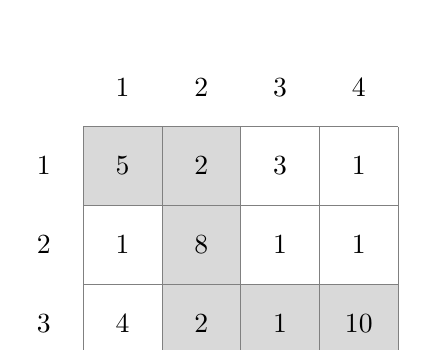
\begin{tikzpicture}
        \fill[gray!30] (0,2) rectangle (1,3);
        \fill[gray!30] (1,2) rectangle (2,3);
        \fill[gray!30] (1,1) rectangle (2,2);
        \fill[gray!30] (1,0) rectangle (2,1);
        \fill[gray!30] (2,0) rectangle (3,1);
        \fill[gray!30] (3,0) rectangle (4,1);

        \draw[gray,very thin] (0,0) grid (4, 3);

        \node at (0.5, 2.5) {5};
        \node at (1.5, 2.5) {2};
        \node at (2.5, 2.5) {3};
        \node at (3.5, 2.5) {1};

        \node at (0.5, 1.5) {1};
        \node at (1.5, 1.5) {8};
        \node at (2.5, 1.5) {1};
        \node at (3.5, 1.5) {1};

        \node at (0.5, 0.5) {4};
        \node at (1.5, 0.5) {2};
        \node at (2.5, 0.5) {1};
        \node at (3.5, 0.5) {10};

        \node at (1.5, 3.5) {2};
        \node at (0.5, 3.5) {1};
        \node at (2.5, 3.5) {3};
        \node at (3.5, 3.5) {4};

        \node at (-0.5, 2.5) {1};
        \node at (-0.5, 1.5) {2};
        \node at (-0.5, 0.5) {3};
    \end{tikzpicture}
    \caption{Exemplo da entrada com células coloridas}
\end{figure}

\vspace{0.3cm}
\textbf{Entrada}

A primeira linha contém dois inteiros $N$ e $M$ ($1 \leq N, M \leq 2000$), representando respectivamente o número de linhas e colunas da grade.

Em seguida, seguem $N$ linhas, cada uma contendo $M$ inteiros $C_{i,j}$ ($0 \leq C_{i,j} \leq 10^4$), representando a quantidade de abóboras em cada posição $i$ e $j$.

\vspace{0.3cm}
\textbf{Saída}

Imprima um único inteiro, sendo o número máximo de abóboras que podem ser colhidas seguindo as regras.

\begin{table}[ht]
    \centering
    \begin{tabular}{|p{7cm}|p{7cm}|}
        \hline
        \begin{center}
            \vspace{-0.3cm}
            \textbf{Exemplos de Entrada}
            \vspace{-0.3cm}
        \end{center} 
         &  
        \begin{center}
            \vspace{-0.3cm}
            \textbf{Exemplos de Saída}
            \vspace{-0.3cm}
        \end{center} \\ \hline
         \texttt{3 4} & \texttt{28} \\
         \texttt{5 2 3 1} & \texttt{} \\
         \texttt{1 8 1 1} & \texttt{} \\
         \texttt{4 2 1 10} & \texttt{} \\
         \hline
    \end{tabular}
    
    \caption{Exemplos de entradas e saídas}
    \label{tab:inputA1}
    
\end{table}

\vspace{0.3cm}

\newpage

\begin{center}
\noindent
\lstinputlisting{abobora_25/A/A5.cpp}
\end{center}
\begin{center}
Problema B

O Desafio do Chocolate do Zé do Grafo

{\small Nome do arquivo: B.c, B.cpp, B.java, ou B.py}

{\large Timelimit: $1$}

{\tiny Por André da Cunha Ribeiro}

\end{center}					

Todo competidor de maratona de programação sabe que as longas horas de um concurso exigem um combustível especial para o cérebro. E qual é o lanche preferido de 10 entre 10 programadores para manter o foco e a energia? Chocolate, é claro! A combinação de açúcar e cafeína parece ter sido feita sob medida para transformar um bug teimoso em um cobiçado "Accepted".

%Zé do Grafo, mais do que um professor, é um mentor que entende perfeitamente a rotina de seus alunos. Vendo sua equipe exausta após um treino intenso para a grande final da competição, ele aparece com o suprimento de energia definitivo: uma enorme barra de chocolate retangular, com N fileiras e M colunas.

%Mas, fiel ao seu estilo, Zé do Grafo não perderia a chance de um bom desafio. Ele colocou a barra de chocolate sobre a mesa e continuou: "O processo para dividir nosso prêmio é simples. A cada movimento, só podemos pegar um único pedaço de chocolate e quebrá-lo uma única vez, sempre em linha reta, seguindo um dos sulcos que dividem os quadrados. Cada quebra transforma um pedaço em dois. Vamos repetir isso até que toda a barra se transforme nos pequenos quadrados individuais de 1x1."

%Ele fez uma pausa e olhou para a equipe com um olhar astuto. "Agora, a pergunta que vale o primeiro pedaço: qual o número exato de quebras necessárias para completar a tarefa?"


Zé do Grafo, um famoso professor de Teoria dos Grafos e um ávido criador de quebra-cabeças, propôs um desafio para seus alunos. Ele apresentou uma barra de chocolate retangular, dividida em pequenos quadrados por sulcos, formando uma grade de $N$ fileiras e $M$ colunas.

O desafio é o seguinte: para dividir a barra de chocolate em $(N * M)$ quadrados de chocolate individuais, os alunos só podem realizar um tipo de movimento. A cada passo, eles podem pegar um único pedaço de chocolate e quebrá-lo ao longo de um dos sulcos (seja na horizontal ou na vertical), resultando em dois pedaços menores.

Sua tarefa é criar um programa que ajude os alunos do Zé do Grafo a descobrir rapidamente o número total de quebras necessárias para transformar a barra inteira em quadrados individuais.

\vspace{0.3cm}
\textbf{Entrada}
A entrada contém  na primeira linha o valor $1 \leq X \leq 1000$ que representa o número dos casos de teste. Seguido de $X$ leituras dos valores de $N,M$ $(1 \leq N,M \leq 10^9)$ indicando as dimensões dos chocolates. 


\vspace{0.3cm}
\textbf{Saída}
Para cada caso de teste, o programa deve produzir uma linha na saída, contendo um único inteiro que representa o número total de quebras necessárias para dividir o chocolate daquele caso de teste.

{\tiny
\begin{table}[h]
    \centering
    \begin{tabular}{|p{7cm}|p{7cm}|}
        \hline
        \begin{center}
            \vspace{-0.3cm}
            \textbf{Exemplos de Entrada}
            \vspace{-0.3cm}
        \end{center} 
         &  
        \begin{center}
            \vspace{-0.3cm}
            \textbf{Exemplos de Saída}
            \vspace{-0.3cm}
        \end{center} \\ \hline
         \texttt{4} & \texttt{3} \\  
         \texttt{2 2} & \texttt{23} \\
         \texttt{4 6} & \texttt{55} \\
         \texttt{7 8} & \texttt{836} \\
         \texttt{27 31} & \texttt{} \\
        \hline
    \end{tabular}
    \caption{Exemplos de entradas e saídas}
\end{table}}

\newpage

\begin{center}
\noindent
\lstinputlisting{abobora_25/B/B5.cpp}
\end{center}

\begin{center}
Problema C

Otimização de Rotas de Coleta de Solo - Simple Smart Agro

{\small Nome do arquivo: C.c, C.cpp, C.java, ou C.py}

{\large Timelimit: $2$}

{\tiny Por Alexandre da Silva}

\end{center}	

\footnotesize
			
A Simple Smart Agro está desenvolvendo um sistema automatizado para coleta de amostras de solo em uma fazenda. O sistema precisa otimizar as rotas de coleta para maximizar a eficiência do processo. Existem $N$ pontos específicos onde amostras de solo devem ser coletadas. O veículo de coleta parte sempre do depósito localizado na origem $(0, 0)$ e deve retornar ao mesmo ponto após coletar todas as amostras. Devido às características do terreno e dos equipamentos, o veículo só pode se mover nas direções cardeais (norte, sul, leste, oeste) e sempre em linha reta entre dois pontos consecutivos da rota. A distância entre dois pontos $(x_1, y_1)$ e $(x_2, y_2)$ é calculada usando a distância Manhattan: $|x_1 - x_2| + |y_1 - y_2|$.

\subsection*{Entrada}

\begin{itemize}
    \item A primeira linha contém um inteiro $N$ $(1 \leq N \leq 10)$, representando o número de pontos de coleta;
    \item As próximas $N$ linhas contêm dois inteiros $x_i$ e $y_i$ $(-1000 \leq x_i, y_i \leq 1000)$, representando as coordenadas do $i$-ésimo ponto de coleta;
       \item Todos os pontos de coleta são distintos entre si;
    \item Nenhum ponto de coleta coincide com a origem $(0,0)$.
\end{itemize}

\subsection*{Saída}

\begin{itemize}
    \item Uma única linha contendo um inteiro: a menor distância total (distância Manhattan) necessária para visitar todos os pontos de coleta e retornar à origem.
\end{itemize}

\subsection*{Exemplos}

\begin{center}
\begin{tabular}{|p{6cm}|p{4cm}|}
\hline
\textbf{Exemplo de Entrada} & \textbf{Exemplo de Saída} \\
\hline
\texttt{3} & \texttt{26} \\
\texttt{2 3} & \\
\texttt{7 1} & \\
\texttt{5 6} & \\
\hline
\texttt{4} & \texttt{42} \\
\texttt{3 4} & \\
\texttt{8 2} & \\
\texttt{12 8} & \\
\texttt{6 10} & \\
\hline
\texttt{1} & \texttt{8} \\
\texttt{2 2} & \\
\hline
\end{tabular}
\end{center}

\subsection*{Explicação do Primeiro Exemplo}

Partindo da origem $(0,0)$, temos os pontos de coleta em $(2,3)$, $(7,1)$ e $(5,6)$.
Uma rota ótima seria:
$(0,0) \rightarrow (2,3) \rightarrow (5,6) \rightarrow (7,1) \rightarrow (0,0)$

Calculando as distâncias:
\begin{itemize}
    \item $(0,0)$ para $(2,3)$: $|2-0| + |3-0| = 2 + 3 = 5$
    \item $(2,3)$ para $(5,6)$: $|5-2| + |6-3| = 3 + 3 = 6$
    \item $(5,6)$ para $(7,1)$: $|7-5| + |1-6| = 2 + 5 = 7$
    \item $(7,1)$ para $(0,0)$: $|0-7| + |0-1| = 7 + 1 = 8$
\end{itemize}

Distância total: $5 + 6 + 7 + 8 = 26$


\newpage

\begin{center}
\noindent
\lstinputlisting{abobora_25/C/C5.cpp}
\end{center}
\begin{center}
Problema D

Agência de Espionagem

{\small Nome do arquivo: D.c, D.cpp, D.java, ou D.py}

{\large Timelimit: $1$}

{\tiny Por Athos José}


\end{center}

A Agência Nacional de Espionagem mantém em seus cofres uma coleção de símbolos secretos, representados por uma sequência de letras. Esses símbolos podem ser reorganizados em qualquer ordem, de forma a formar novas mensagens.

Agentes inimigos, porém, estão tentando criar mensagens escondidas dentro dessas reorganizações. Uma mensagem inimiga é considerada possível se puder aparecer como uma sequência contínua de caracteres de alguma permutação dos símbolos guardados no cofre.

Sua missão é, para cada mensagem inimiga recebida, determinar se ela pode ser formada a partir dos símbolos da Agência.

\vspace{0.3cm}
\textbf{Entrada}

A primeira linha contém um inteiro $N$ ($1 \leq N \leq 10^5$), o número de mensagens inimigas a serem analisadas, seguido de uma string $S$ ($1 \leq |S| \leq 10^5$) representando os símbolos secretos do cofre.

Cada uma das próximas $N$ linhas contém uma string $Q_i$ ($1 \leq |Q_i| \leq 10^5$), representando uma mensagem inimiga a ser verificada.

A soma dos comprimentos de todas as mensagens $Q_i$ não excede $10^9$.

Todas as strings são compostas apenas de letras minúsculas do alfabeto inglês (a-z).

\vspace{0.3cm}
\textbf{Saída}

Para cada mensagem $Q_i$ imprima uma linha contendo:
\begin{itemize}
    \item ``SIM'', se a mensagem pode ser formada como substring de alguma permutação de $S$.
    \item ``NAO'',caso contrário.
\end{itemize}

\begin{table}[h]
    \centering
    \begin{tabular}{|p{7cm}|p{7cm}|}
       \hline
        \begin{center}
            \vspace{-0.3cm}
            \textbf{Exemplos de Entrada}
            \vspace{-0.3cm}
        \end{center} 
         &  
        \begin{center}
            \vspace{-0.3cm}
            \textbf{Exemplos de Saída}
            \vspace{-0.3cm}
        \end{center} \\ \hline
         \texttt{3 abac} & \texttt{SIM} \\  
         \texttt{caa} & \texttt{NAO} \\
         \texttt{aaa} & \texttt{SIM} \\  
         \texttt{bac} & \\
         \hline
    \end{tabular}
    \caption{Exemplos de entradas e saídas}
    \label{tab:inputB}
\end{table}

\newpage

\begin{center}
\noindent
\lstinputlisting{abobora_25/D/D5.cpp}
\end{center}
\begin{center}
Problema E

Estória da Estônia

{\small Nome do arquivo: E.c, E.cpp, E.java, ou E.py}

{\large Timelimit: $1$}

{\tiny Por Márcio Belo}

\end{center}			

O professor Márcio Belo sempre gostou de charadas matemáticas. Um dia ele se deparou com uma estória, pra lá da Estônia. Dado um número primo ímpar $p$, sempre é possível um triângulo de lados inteiros $x$, $y$ e $z$, em ordem crescente de tamanho com as seguintes propriedades: 
\begin{itemize}
    \item A diferença da soma dos lados menores do triângulo pelo lado maior é igual ao primo $p$; 
    \item A diferença da soma das áreas dos quadrados de lados $x$ e $y$ e a área do quadrado de lado $z$ é igual ao primo $p$. 
\end{itemize}
Em matematiquês:

\vspace{3mm}
Dado um primo $p \geq 3$, sempre existem triplas $(x,y,z)$, com $x \leq y \leq z$ que satisfazem: 
\begin{align*}
    x + y - z & = p \\
    x^{2} + y^{2} - z^{2} & = p 
\end{align*}
Quem são essas triplas $(x,y,z)$? Você pode ajudar o professor?

\vspace{0.3cm}
\textbf{Entrada}
Cada entrada contém uma única linha com o número primo $p$, com $(3 \leq p < 2^{16})$. 

\vspace{0.3cm}
\textbf{Saída}
O sistema deve retornar todas as triplas $(x,y,z)$ em ordem crescente de $x$. Uma tripla por linha,  

\begin{table}[h]
    \centering
    \begin{tabular}{|p{7cm}|p{7cm}|}
        \hline
        \begin{center}
            \vspace{-0.3cm}
            \textbf{Exemplos de Entrada}
            \vspace{-0.3cm}
        \end{center} 
         &  
        \begin{center}
            \vspace{-0.3cm}
            \textbf{Exemplos de Saída}
            \vspace{-0.3cm}
        \end{center} \\ \hline
         \texttt{3} & \texttt{(4,6,7)} \\  
         \hline
         \texttt{5} & \texttt{(6, 15, 16)} \\ 
          & \texttt{(7, 10, 12)} \\ 
         \hline
         \texttt{13} & \texttt{(14, 91, 92)} \\
         & \texttt{(15, 52, 54)} \\
         & \texttt{(16, 39, 42)} \\
         & \texttt{(19, 26, 32)} \\ 
         \hline
         \texttt{65267} & \texttt{(65268,2129923278,2129923279)} \\ 
          & \texttt{(97900,130534,163167)} \\ 
         \hline
    \end{tabular}
    \caption{Exemplos de entradas e saídas}

\end{table}

\newpage
\begin{center}
\noindent
\lstinputlisting{abobora_25/E/E5.cpp}
\end{center}
\begin{center}
Problema F

Monitorando Pragas

{\small Nome do arquivo: F.c, F.cpp, F.java, ou F.py}

{\large Timelimit: $1$}

{\tiny Por Emanuel Silva Araujo}

\end{center}

\footnotesize

O agricultor Seu Jayme sofre constantemente com infestações de insetos em sua lavoura de soja. Para reduzir perdas e otimizar o manejo, ele procurou a EMBRAPII para desenvolver uma ferramenta de monitoramento diário de pragas.
Sua tarefa como programador é implementar um programa que leia os valores de população diária e identifique situações de risco, emitindo alertas de acordo com os seguintes critérios:
%Critérios de Alerta
    \begin{itemize}
        \item  Alerta por pico diário [Pico]
        \begin{itemize}
            \item Se em qualquer dia a população registrada ultrapassar 200 insetos.
        \end{itemize}
        \item  Alerta por variação em 7 dias [7 Dias]
        \begin{itemize}
            \item Se a diferença percentual entre o valor mínimo e o máximo em um intervalo de 7 dias consecutivos for maior ou igual a 20\%.
        \end{itemize}
        \item  Alerta por crescimento contínuo [Crescimento]
        \begin{itemize}
            \item Se ocorrerem 4 dias seguidos de crescimento, e em cada dia a população for pelo menos 5\% maior que a do dia anterior.
        \end{itemize}
    \end{itemize}
        
\vspace{0.3cm}
\textbf{Entrada}

Um número inteiro $(0 <= N <= 360)$, representando a quantidade de dias monitorados (entre os dias $0$ e $360$).
Uma sequência de $N$ números inteiros $(0 < X <= 5000)$, cada um representando a estimativa da população de insetos no respectivo dia.

\vspace{0.3cm}
\textbf{Saída}

    Para cada alerta identificado, o programa deve imprimir:
    \begin{itemize}
        \item O tipo do alerta;
        \item O(s) dia(s) correspondente(s);
        \item O valor percentual (quando aplicável), com duas casas decimais.
    \end{itemize}
    Caso não tenha nenhum alerta, deve imprimir uma mensagem de "Nenhum Alerta".
    Para dias que tiveram mais de um alerta a ordem de impressão é: $[Pico] > [7 Dias] > [Crescimento]$.
 
\begin{table}[h]
    \centering
    \footnotesize
    \begin{tabular}{|p{8cm}|p{8cm}|}
        \hline
        \begin{center}
            \vspace{-0.3cm}
            \textbf{Exemplos de Entrada}
            \vspace{-0.3cm}
        \end{center} 
         &  
        \begin{center}
            \vspace{-0.3cm}
            \textbf{Exemplos de Saída}
            \vspace{-0.3cm}
        \end{center} \\ \hline
		    \texttt{10} & \texttt{[Crescimento] 1-4: maior que >= 5\% } \\
                \texttt{50 60 70 80 90 200 210 220 180 170} & \texttt{[Crescimento] 1-5: maior que >= 5\% } \\
& \texttt{[Crescimento] 1-6: maior que >= 5\% } \\
& \texttt{[Pico] 7: 210 insetos} \\
& \texttt{[7 Dias] 1-7: 320.00\%} \\
& \texttt{[Crescimento] 1-7: maior que >= 5\% } \\
& \texttt{[Pico] 8: 220 insetos} \\
& \texttt{[7 Dias] 2-8: 266.67\%} \\
& \texttt{[7 Dias] 3-9: 214.29\%} \\
& \texttt{[7 Dias] 4-10: 175.00\%} \\


         \hline
   		    \texttt{9}   & \texttt{[Crescimento] 1-4: maior que >= 5\% } \\
            \texttt{100 105 112 118 90 96 100 120 80} & \texttt{[7 Dias] 2-8: 33.33\%} \\
         \hline    
   		    \texttt{8}   & \texttt{Nenhum Alerta} \\
            \texttt{118 120 118 140 140 140 130 100} & \\
         \hline    
    \end{tabular}
    \caption{Exemplos de entradas e saídas}

\end{table}

\normalsize

\newpage

\begin{center}
\lstinputlisting{abobora_25/F/F5.cpp}
\end{center}

\begin{center}
Problema G

Comportamento Dinâmico

{\small Nome do arquivo: G.c, G.cpp, G.java, ou G.py}

{\large Timelimit: $1$}

{\tiny Por Heverton Barros de Macêdo}

\end{center}

\footnotesize

	Durante uma investigação sobre o comportamento de sistemas dinâmicos, Wolfram definiu o seguinte cenário para efetuar experimentos: dada uma cadeia de $N$ células, linearmente distribuídas, cada célula armazena um único estado (bit), e além disso as células das extremidades são vizinhas entre si. Para cada instante de tempo $t$ a evolução dessa cadeia ocorre simultaneamente em todas as células, considerando uma regra de evolução previamente definida. Essa regra é aplicada a cada vizinhança de $K=3$ células gerando um novo estado, conforme indicado na Tabela~\ref{tab:evolucao}.
	
	\begin{table}[h!]
		\caption{Regra aplicada para evolução do experimento de Wolfram.}
		\label{tab:evolucao}
		
		\centering
		\footnotesize{
		\begin{tabular}{|c|c|c|c|c|c|c|c|c|}
			\hline
			\cellcolor[HTML]{DDDDDD} Regra para vizinhança & 000 & 001 & \cellcolor[HTML]{FFAAAA} 010 & 011 & 100 & 101 & 110 & 111 \\ \hline
			\cellcolor[HTML]{DDDDDD} Novo estado para célula central & 1 & 0 &  \cellcolor[HTML]{AAFFAA} 0 & 1 & 0 & 0 & 0 & 1 \\ \hline
		\end{tabular}
		}
	\end{table}

Como exemplo, considere um experimento (veja a Tabela~\ref{tab:exemplo_evolucao}) com a cadeia de bits formada por $11$ células ($N = 11$), em que no instante $t = 0$ apenas um bit, exatamente no centro da cadeia, possui o estado $1$ e as demais células possuem o estado $0$, evoluindo por $4$ passos de tempo ($t = 4$).
%Como exemplo, considere um experimento (veja a Tabela~\ref{tab:exemplo_evolucao}) com a cadeia de bits no espaço linear formada por $11$ células ($N = 11$), em que apenas um bit, exatamente no centro da cadeia ($t = 0$), possui o estado $1$ e as demais células possuem o estado $0$, evoluindo por $4$ passos de tempo.

A Tabela~\ref{tab:exemplo_evolucao} ilustra o experimento com a configuração inicial ($t = 0$) formada por: $00000100000$. No próximo passo de tempo ($t = 1$), todas as células evoluem (podem alterar o estado) considerando a vizinhança indicada na regra (Tabela~\ref{tab:evolucao}). Em destaque na cor vermelha (Tabelas~\ref{tab:evolucao} e ~\ref{tab:exemplo_evolucao}) está a atualização da célula central, formada pela vizinhança $010$ que, segundo a regra, deve evoluir no próximo passo de tempo ($t = 1$) para o estado $0$ (destaque na cor verde). É possível notar no exemplo, a evolução da cadeia inicial por $4$ passos de tempo. Vale destacar que as células na extremidade (esquerda e direta) estão conectadas (formato de anel - toroidal)

	\begin{table}[h!]
	\caption{Exemplo de um experimento por $4$ passos de tempo.}
	\label{tab:exemplo_evolucao}
	
	\centering
	\footnotesize{	
	\begin{tabular}{|c|c|c|c|c|c|c|c|c|c|c|c|}
		\hline
		Tempo & \multicolumn{11}{c|}{Cadeia linear de N células}\\ \hline
    	$t = 0$ & 0 & 0 & 0 & 0 & \cellcolor[HTML]{FFAAAA} 0 & \cellcolor[HTML]{FFAAAA} 1 & \cellcolor[HTML]{FFAAAA} 0 & 0 & 0 & 0 & 0 \\ \hline
		$t = 1$ & 1 & 1 & 1 & 1 &  0 & \cellcolor[HTML]{AAFFAA} 0 & 0 & 1 & 1 & 1 & 1 \\ \hline
		$t = 2$ & 1 & 1 & 1 & 0 &  1 & 0 & 0 & 1 & 1 & 1 & 1 \\ \hline
		$t = 3$ & 1 & 1 & 0 & 0 &  0 & 0 & 0 & 1 & 1 & 1 & 1 \\ \hline
		$t = 4$ & 1 & 0 & 0 & 1 &  1 & 1 & 0 & 1 & 1 & 1 & 1 \\ \hline
	\end{tabular}
	}	
\end{table}

%\pagebreak
Sua missão é ajudar Wolfram a obter a configuração dos estados após $t$ passos de tempo, considerando uma
sequência inicial qualquer no tempo $t = 0$ e a aplicação da regra indicada no enunciado.

\vspace{0.3cm}
\textbf{Entrada}

A entrada contém vários casos de teste. Cada linha contém um inteiro $t$ ($0~<~t~\leq~1000$), que representa
a quantidade de passos de evolução, seguido pela cadeia de bits no tempo $t = 0$, que pode variar conforme a
quantidade de células da amostra $N$ ($3 \leq N < 100$).

\vspace{0.3cm}
\textbf{Saída}

O programa deve produzir como saída a configuração da cadeia no espaço linear de células após a evolução
de $t$ passos de tempo.

\begin{table}[h]
    \centering
    \footnotesize
    \begin{tabular}{|p{8cm}|p{8cm}|}
        \hline
        \begin{center}
            \vspace{-0.3cm}
            \textbf{Exemplos de Entrada}
            \vspace{-0.3cm}
        \end{center} 
         &  
        \begin{center}
            \vspace{-0.3cm}
            \textbf{Exemplos de Saída}
            \vspace{-0.3cm}
        \end{center} \\ \hline
		    \texttt{1 00000100000} & \texttt{11110001111} \\
         \hline
   		    \texttt{2 00000100000} & \texttt{11100101111} \\
         \hline    
   		    \texttt{3 00000100000} & \texttt{11000001111} \\
         \hline    
   		    \texttt{578 00000100000} & \texttt{00000111101} \\
         \hline    
   		    \texttt{978 011001111000110111010011} & \texttt{100111000001110000011101} \\
         \hline    
    \end{tabular}
    \caption{Exemplos de entradas e saídas}    
\end{table}

\normalsize

\newpage

\begin{center}
\noindent
\lstinputlisting{abobora_25/G/G5.cpp}
\end{center}
\begin{center}
Problema H

Josephus das Abóboras

{\small Nome do arquivo: H.c, H.cpp, H.java, ou H.py}

{\large Timelimit: $1$}

{\tiny Por Heverton Barros de Macêdo}

\end{center}

{\footnotesize
Finalmente chegou o dia das bruxas e os “corajosos” estudantes de Ciência da Computação estão prontos para adentrar no castelo mal-assombrado. O problema é que a porta do castelo é muito estreita e permite que apenas um estudante adentre por vez. Como todos estão com medo, Josephus decidiu fazer um sorteio para estabelecer a ordem em que eles devem entrar. A seguinte regra foi estabelecida:

\begin{enumerate}
    \item Os estudantes devem se posicionar em formato de círculo;
    \item Cada estudante apresenta um número com os dedos da mão;
    \item Faz-se a soma dos números e define o resultado como X;
    \item A contagem dos estudantes é iniciada em zero a partir do primeiro estudante adicionado no círculo, seguindo em sentido horário. Quando a contagem atingir X, o estudante daquela posição será escolhido como o primeiro a ingressar no castelo.
    \item O estudante seguinte ao escolhido, servirá como ponto de partida para a nova contagem até o número X, que determina o próximo a ingressar no castelo.
    \item O passo anterior deverá ser repetido até que reste apenas um estudante, momento em que a sequência é finalizada, definindo o último aluno a ingressar no castelo.
\end{enumerate}

Como exemplo, considere os estudantes: Fulano, Beltrano, Sicrano e Josephus. A disposição dos estudantes colocando-os em círculo pode ser visualizada na Figura \ref{figura:h1}.

\begin{figure}[!ht]
\centering

\includegraphics[width=8cm]{fig/h_1.png}
\caption{Disposição inicial em formato circular}
\label{figura:h1}
\end{figure}

Considere que a soma dos números dos dedos da mão indicados pelos estudantes seja 7 $(X = 7)$. Fazendo a contagem no sentido horário, partindo de Fulano, temos: Beltrano (1), Sicrano (2), Josephus (3), Fulano (4), continuando o círculo, Beltrano (5), Sicrano (6), Josephus (7). A Figura \ref{figura:h2} ilustra a contagem, destacando o número 7 em vermelho como sendo o estudante a ser removido do círculo.

\begin{figure}[!htbp]
\centering

\includegraphics[width=8cm]{fig/h_2.png}
\caption{Contagem considerando o número $X = 7$ e o aluno Fulano como referência para o início da contagem}
\label{figura:h2}
\end{figure}

Para essa rodada o Josephus foi selecionado como primeiro a ingressar no castelo. Considerando Josephus fora do círculo, iniciamos novamente a contagem a partir do próximo do círculo (coincidentemente Fulano). Na sequência temos: Beltrano (1), Sicrano (2), Fulano (3), Beltrano (4), Sicrano (5), Fulano (6), Beltrano (7), indicando que Beltrano é o segundo a adentrar no Castelo. Continuando o sorteio com Beltrano fora do círculo e a contagem iniciando de Sicrano (próximo no sentido horário) teremos: Fulano (1), Sicrano (2), Fulano (3), Sicrano (4), Fulano (5), Sicrano (6), Fulano (7). Por fim, temos a sequência de estudantes a entrar no castelo: Josephus, Beltrano, Fulano e Sicrano.

Sua missão é ajudar Josephus a obter a sequência correta para adentrar ao castelo, independente do número de estudantes que estiver o acompanhando.

\vspace{0.3cm}
\textbf{Entrada:}
A entrada contém vários casos de teste. A primeira linha de cada caso contém os nomes dos estudantes separados com um espaço. A segunda linha contém o número inteiro X $(1 \leq X \leq 10.000)$ que será usado para a contagem (Obs: para cada nome não deve haver espaço e haverá no máximo 20 caracteres. Exemplo de nome inválido: "João da Silva". Exemplo de nome válido "JoãodaSilva").

\vspace{0.3cm}
\textbf{Saída:}
O programa deve produzir como saída a sequência de nomes a adentrar no castelo separados por um espaço (Obs: Ao término do último nome da lista não deve haver espaço, somente o terminador de linha).

\begin{table}[!htbp]
    \centering
    \begin{tabular}{|p{8cm}|p{7cm}|}
        \hline
        \begin{center}
            \vspace{-0.3cm}
            \textbf{Exemplos de Entrada}
            \vspace{-0.3cm}
        \end{center} 
         &  
        \begin{center}
            \vspace{-0.3cm}
            \textbf{Exemplos de Saída}
            \vspace{-0.3cm}
        \end{center} \\ \hline
         \texttt{Fulano Sicrano} & \texttt{Sicrano Fulano} \\  
         \texttt{1} & \texttt{} \\  
         \hline
         \texttt{Fulano Sicrano Beltrano} & \texttt{Sicrano Fulano Beltrano} \\  
         \texttt{1} & \texttt{} \\  
         \hline    
         \texttt{Fulano Sicrano Beltrano} & \texttt{Beltrano Fulano Sicrano} \\  
         \texttt{2} & \texttt{} \\  
         \hline
         \texttt{Fulano Sicrano Beltrano} & \texttt{Fulano Sicrano Beltrano} \\  
         \texttt{6} & \texttt{} \\  
         \hline
         \texttt{Fulano Beltrano Sicrano Josephus} & \texttt{Josephus Beltrano Fulano Sicrano} \\  
         \texttt{7} & \texttt{} \\  
         \hline 
    \end{tabular}
    \caption{Exemplos de entradas e saídas}
    \label{tab:inputHProblem24}
\end{table}}

\newpage

\begin{center}
\noindent
\lstinputlisting{abobora_24/H/H4.cpp}
\end{center}
\begin{center}
Problema I

Heverton e a Fila 

{\tiny by André da Cunha Ribeiro}

Timelimit: $1$	
\end{center}			

Heverton é um coordenador de curso muito dedicado do curso de computação do NuCAT. Os alunos estão enfrentando um grande problema na entrada do NuCAT, todos querem entrar no mesmo horário gerando assim um grande tumulto. Heverton reuniu com os cavalheiros do NDE para tentar resolver o problema. Depois de muita discussão o NDE resolveu ordenar os alunos pelo número de matricula, e organizando a entrada pela ordem decrescente. Mas Heverton precisa de sua ajuda para desenvolver o programa pois ele está muito ocupado com seus trabalhos.

\vspace{0.3cm}
\textbf{Entrada}
Para cada dia será lido um inteiro $N$, $1 \leq  N  \leq  10^{4}$, que representa o número de alunos disponíveis na entrada. Depois será lido os $N$ números de matriculas.

\vspace{0.3cm}
\textbf{Saída}
Para cada dia, imprimir os  número de  matriculas ordenados em ordem decrescente.

\begin{table}[h]
    \centering
    \begin{tabular}{|p{7cm}|p{7cm}|}
        \hline
        \begin{center}
            \vspace{-0.3cm}
            \textbf{Exemplos de Entrada}
            \vspace{-0.3cm}
        \end{center} 
         &  
        \begin{center}
            \vspace{-0.3cm}
            \textbf{Exemplos de Saída}
            \vspace{-0.3cm}
        \end{center} \\ \hline
         \texttt{5} & \texttt{5 4 3 2 1} \\  
         \texttt{1 2 3 4 5} & \texttt{} \\
         \hline
    \end{tabular}
    \caption{Exemplos de entradas e saídas}
    \label{tab:inputI2}
\end{table}

\newpage

\begin{center}
\noindent
\lstinputlisting{abobora_23/I/I3.cpp}
\end{center}

\begin{center}
Problema J

Zé do Grafo

{\tiny Por André da Cunha Ribeiro}

Timelimit: $1$	
\end{center}			

{\footnotesize
Zé do Grafo, a lenda que ecoa como o Mestre Jedi exterminador de monstros, emerge das sombras como uma faísca ardente de esperança na enigmática cidade entrelaçada nos recônditos do IFGoiano - Campus Rio Verde. Essa cidade, envolta em mistério, desdobra-se perante olhares curiosos como um enigma arquitetônico complexo, com conexões intrincadas que aguçam a mente.

Nesse ambiente intrigante, Zé do Grafo se ergue como um guardião destemido, dotado de poderes transcendentes. Em um dia sereno, enquanto explorava a cidade, ele desvenda um bairro oculto, um santuário de portais secretos que se estendem ao multiverso. Cada portal é adornado com inscrições enigmáticas, revelando as delicadas ligações entre os diversos universos. Uma característica única surge: cada universo conectado é tingido por uma cor distinta, representando a natureza de sua atmosfera. Nota-se que universos vizinhos exibem atmosferas diversas, delineando uma dança cósmica de elementos distintos.

Entretanto, dilemas pairam sobre Zé do Grafo: ele só pode sobreviver em dois tipos específicos de atmosfera, uma limitação impregnada pelas superstições que permeiam a linhagem de mestres Jedi. A narrativa então faz um compasso, direcionando o holofote para um novo protagonista: você. Sua ajuda, inestimável e ancorada na compreensão profunda dos algoritmos e grafos, é convocado para solucionar este enigma vital. A pergunta que se insinua é crucial: há algum portal capaz de permitir que o lendário Zé do Grafo explore os multiversos, sem que isso desafie suas crenças enraizadas na superstição?

\vspace{0.3cm}
\textbf{Entrada}
Cada entrada contém os dados de cada portal. A primeira linha contém dois inteiros $N$, $M$, indicando respectivamente o número de multiversos $(1 \leq N \leq 50)$ e as ligações dos multiversos $(1 \leq M \leq 2000)$.

Cada uma das $M$ linhas seguintes composta de dois inteiros que descreve as ligações dos multiverso.

\vspace{0.3cm}
\textbf{Saída}
O sistema deve retornar ``Sim'' caso Zé do Grafos consiga explorar todo o multiverso. Caso contrário, a resposta será ``Não''.
\begin{table}[h]
    \centering
    \begin{tabular}{|p{7cm}|p{7cm}|}
        \hline
        \begin{center}
            \vspace{-0.3cm}
            \textbf{Exemplos de Entrada}
            \vspace{-0.3cm}
        \end{center} 
         &  
        \begin{center}
            \vspace{-0.3cm}
            \textbf{Exemplos de Saída}
            \vspace{-0.3cm}
        \end{center} \\ \hline
         \texttt{6 7} & \texttt{Sim} \\  
         \texttt{1 2} & \texttt{} \\
         \texttt{1 6} & \texttt{} \\
         \texttt{2 3} & \texttt{} \\
         \texttt{3 4} & \texttt{} \\
         \texttt{3 6} & \texttt{} \\
         \texttt{4 5} & \texttt{} \\         
         \texttt{5 6} & \texttt{} \\
         \hline
         \texttt{6 7} & \texttt{Não} \\  
         \texttt{1 2} & \texttt{} \\
         \texttt{1 3} & \texttt{} \\
         \texttt{2 3} & \texttt{} \\
         \texttt{3 4} & \texttt{} \\
         \texttt{4 5} & \texttt{} \\
         \texttt{4 6} & \texttt{} \\
         \texttt{5 6} & \texttt{} \\
         \hline
         \texttt{3 3} & \texttt{Não} \\  
         \texttt{1 2} & \texttt{} \\
         \texttt{1 3} & \texttt{} \\
         \texttt{2 3} & \texttt{} \\
         \hline
    \end{tabular}
    \caption{Exemplos de entradas e saídas}
    \label{tab:inputJJ}
\end{table}}

\newpage

\begin{center}
\noindent
\lstinputlisting{abobora_23/J/J3.cpp}
\end{center}




\begin{center}
 {\large {\textbf 
5º Abóbora Contest}}

%Sub-Regional Brasil do ACM ICPC

{\large 31 de Outubro de 2024}

{\large  Caderno de Problemas}

{\large \textbf{Informações Gerais}}
\end{center}

Este caderno contém $8$ problemas; as páginas estão numeradas de $1$ a $10$,  contando esta página de rosto. Verifique se o caderno está completo.

\begin{enumerate}
    \item \textbf{Sobre os nomes dos programas}
    \begin{enumerate}
        \item Para soluções em C/C++ e Python 3.10, o nome do arquivo-fonte não é significativo, pode ser qualquer nome desde que tenha as extensões .c, .cpp, .java e .py.
        \item Para linguagem Java, sua solução deve ser chamado de codigo\_do\_problema.java, em que codigo\_do\_problema é a letra maiúscula que identifica o problema. Lembre que em Java o nome da classe principal deve ser igual ao nome do arquivo.
    \end{enumerate}
    \item \textbf{Sobre a entrada}
    \begin{enumerate}
        \item A entrada de seu programa deve ser lida da entrada padrão.
        \item A entrada é composta de um único caso de teste, descrito em um número de linhas que depende do problema.
        \item Quando uma linha da entrada contém vários valores, estes são separados por um único espaço em branco; a entrada não contém nenhum outro espaço em branco.
        \item Cada linha, incluindo a última, contém exatamente um caractere final-de-linha.
        \item O final da entrada coincide com o final do arquivo.
    \end{enumerate}
    \item \textbf{Sobre a saída}
    \begin{enumerate}
        \item A saída de seu programa deve ser escrita na saída padrão.
        \item Quando uma linha da saída contém vários valores, estes devem ser separados por um único espaço em branco; a saída não deve conter nenhum outro espaço em branco.
        \item Cada linha, incluindo a última, deve conter exatamente um caractere final-de-linha.
    \end{enumerate}
\end{enumerate}

\newpage
\begin{center}
Problema A

Caminho da Colheita

{\small Nome do arquivo: A.c, A.cpp, A.java, ou A.py}

{\large Timelimit: $1$}

{\tiny Por Athos José}

\end{center}

Seu Zé, fazendeiro importante de Rio Verde tem uma plantação de abóboras organizadas em uma área retangular de tamanho $N$ x $M$, cada muda de abóbora está em uma área $1$x$1$ e contém uma certa quantidade de abóboras.

Costumeiramente, Seu Zé faz a colheita em um percurso único, começando no canto superior esquerdo do campo (posição ($1,1$)) e termina sempre no canto inferior direito do campo ($N,M$). A cada passo, ele mover-se apenas para a direita ou para baixo.

A plantação de Seu Zé cresceu muito e acredita que o carinho que usa para colher não é suficientemente grande para acomodar todas as abóboras no caminho. Agora ele pediu sua ajuda para que dado o campo informa-se qual é máximo de abóboras possível de colher ao longo do melhor caminho.

\vspace{0.3cm}
\begin{figure}[h]
    \centering
    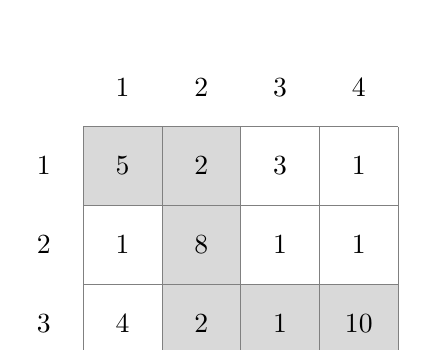
\begin{tikzpicture}
        \fill[gray!30] (0,2) rectangle (1,3);
        \fill[gray!30] (1,2) rectangle (2,3);
        \fill[gray!30] (1,1) rectangle (2,2);
        \fill[gray!30] (1,0) rectangle (2,1);
        \fill[gray!30] (2,0) rectangle (3,1);
        \fill[gray!30] (3,0) rectangle (4,1);

        \draw[gray,very thin] (0,0) grid (4, 3);

        \node at (0.5, 2.5) {5};
        \node at (1.5, 2.5) {2};
        \node at (2.5, 2.5) {3};
        \node at (3.5, 2.5) {1};

        \node at (0.5, 1.5) {1};
        \node at (1.5, 1.5) {8};
        \node at (2.5, 1.5) {1};
        \node at (3.5, 1.5) {1};

        \node at (0.5, 0.5) {4};
        \node at (1.5, 0.5) {2};
        \node at (2.5, 0.5) {1};
        \node at (3.5, 0.5) {10};

        \node at (1.5, 3.5) {2};
        \node at (0.5, 3.5) {1};
        \node at (2.5, 3.5) {3};
        \node at (3.5, 3.5) {4};

        \node at (-0.5, 2.5) {1};
        \node at (-0.5, 1.5) {2};
        \node at (-0.5, 0.5) {3};
    \end{tikzpicture}
    \caption{Exemplo da entrada com células coloridas}
\end{figure}

\vspace{0.3cm}
\textbf{Entrada}

A primeira linha contém dois inteiros $N$ e $M$ ($1 \leq N, M \leq 2000$), representando respectivamente o número de linhas e colunas da grade.

Em seguida, seguem $N$ linhas, cada uma contendo $M$ inteiros $C_{i,j}$ ($0 \leq C_{i,j} \leq 10^4$), representando a quantidade de abóboras em cada posição $i$ e $j$.

\vspace{0.3cm}
\textbf{Saída}

Imprima um único inteiro, sendo o número máximo de abóboras que podem ser colhidas seguindo as regras.

\begin{table}[ht]
    \centering
    \begin{tabular}{|p{7cm}|p{7cm}|}
        \hline
        \begin{center}
            \vspace{-0.3cm}
            \textbf{Exemplos de Entrada}
            \vspace{-0.3cm}
        \end{center} 
         &  
        \begin{center}
            \vspace{-0.3cm}
            \textbf{Exemplos de Saída}
            \vspace{-0.3cm}
        \end{center} \\ \hline
         \texttt{3 4} & \texttt{28} \\
         \texttt{5 2 3 1} & \texttt{} \\
         \texttt{1 8 1 1} & \texttt{} \\
         \texttt{4 2 1 10} & \texttt{} \\
         \hline
    \end{tabular}
    
    \caption{Exemplos de entradas e saídas}
    \label{tab:inputA1}
    
\end{table}

\vspace{0.3cm}

\newpage

\begin{center}
\noindent
\lstinputlisting{abobora_25/A/A5.cpp}
\end{center}
\begin{center}
Problema B

O Desafio do Chocolate do Zé do Grafo

{\small Nome do arquivo: B.c, B.cpp, B.java, ou B.py}

{\large Timelimit: $1$}

{\tiny Por André da Cunha Ribeiro}

\end{center}					

Todo competidor de maratona de programação sabe que as longas horas de um concurso exigem um combustível especial para o cérebro. E qual é o lanche preferido de 10 entre 10 programadores para manter o foco e a energia? Chocolate, é claro! A combinação de açúcar e cafeína parece ter sido feita sob medida para transformar um bug teimoso em um cobiçado "Accepted".

%Zé do Grafo, mais do que um professor, é um mentor que entende perfeitamente a rotina de seus alunos. Vendo sua equipe exausta após um treino intenso para a grande final da competição, ele aparece com o suprimento de energia definitivo: uma enorme barra de chocolate retangular, com N fileiras e M colunas.

%Mas, fiel ao seu estilo, Zé do Grafo não perderia a chance de um bom desafio. Ele colocou a barra de chocolate sobre a mesa e continuou: "O processo para dividir nosso prêmio é simples. A cada movimento, só podemos pegar um único pedaço de chocolate e quebrá-lo uma única vez, sempre em linha reta, seguindo um dos sulcos que dividem os quadrados. Cada quebra transforma um pedaço em dois. Vamos repetir isso até que toda a barra se transforme nos pequenos quadrados individuais de 1x1."

%Ele fez uma pausa e olhou para a equipe com um olhar astuto. "Agora, a pergunta que vale o primeiro pedaço: qual o número exato de quebras necessárias para completar a tarefa?"


Zé do Grafo, um famoso professor de Teoria dos Grafos e um ávido criador de quebra-cabeças, propôs um desafio para seus alunos. Ele apresentou uma barra de chocolate retangular, dividida em pequenos quadrados por sulcos, formando uma grade de $N$ fileiras e $M$ colunas.

O desafio é o seguinte: para dividir a barra de chocolate em $(N * M)$ quadrados de chocolate individuais, os alunos só podem realizar um tipo de movimento. A cada passo, eles podem pegar um único pedaço de chocolate e quebrá-lo ao longo de um dos sulcos (seja na horizontal ou na vertical), resultando em dois pedaços menores.

Sua tarefa é criar um programa que ajude os alunos do Zé do Grafo a descobrir rapidamente o número total de quebras necessárias para transformar a barra inteira em quadrados individuais.

\vspace{0.3cm}
\textbf{Entrada}
A entrada contém  na primeira linha o valor $1 \leq X \leq 1000$ que representa o número dos casos de teste. Seguido de $X$ leituras dos valores de $N,M$ $(1 \leq N,M \leq 10^9)$ indicando as dimensões dos chocolates. 


\vspace{0.3cm}
\textbf{Saída}
Para cada caso de teste, o programa deve produzir uma linha na saída, contendo um único inteiro que representa o número total de quebras necessárias para dividir o chocolate daquele caso de teste.

{\tiny
\begin{table}[h]
    \centering
    \begin{tabular}{|p{7cm}|p{7cm}|}
        \hline
        \begin{center}
            \vspace{-0.3cm}
            \textbf{Exemplos de Entrada}
            \vspace{-0.3cm}
        \end{center} 
         &  
        \begin{center}
            \vspace{-0.3cm}
            \textbf{Exemplos de Saída}
            \vspace{-0.3cm}
        \end{center} \\ \hline
         \texttt{4} & \texttt{3} \\  
         \texttt{2 2} & \texttt{23} \\
         \texttt{4 6} & \texttt{55} \\
         \texttt{7 8} & \texttt{836} \\
         \texttt{27 31} & \texttt{} \\
        \hline
    \end{tabular}
    \caption{Exemplos de entradas e saídas}
\end{table}}

\newpage

\begin{center}
\noindent
\lstinputlisting{abobora_25/B/B5.cpp}
\end{center}

\begin{center}
Problema C

Otimização de Rotas de Coleta de Solo - Simple Smart Agro

{\small Nome do arquivo: C.c, C.cpp, C.java, ou C.py}

{\large Timelimit: $2$}

{\tiny Por Alexandre da Silva}

\end{center}	

\footnotesize
			
A Simple Smart Agro está desenvolvendo um sistema automatizado para coleta de amostras de solo em uma fazenda. O sistema precisa otimizar as rotas de coleta para maximizar a eficiência do processo. Existem $N$ pontos específicos onde amostras de solo devem ser coletadas. O veículo de coleta parte sempre do depósito localizado na origem $(0, 0)$ e deve retornar ao mesmo ponto após coletar todas as amostras. Devido às características do terreno e dos equipamentos, o veículo só pode se mover nas direções cardeais (norte, sul, leste, oeste) e sempre em linha reta entre dois pontos consecutivos da rota. A distância entre dois pontos $(x_1, y_1)$ e $(x_2, y_2)$ é calculada usando a distância Manhattan: $|x_1 - x_2| + |y_1 - y_2|$.

\subsection*{Entrada}

\begin{itemize}
    \item A primeira linha contém um inteiro $N$ $(1 \leq N \leq 10)$, representando o número de pontos de coleta;
    \item As próximas $N$ linhas contêm dois inteiros $x_i$ e $y_i$ $(-1000 \leq x_i, y_i \leq 1000)$, representando as coordenadas do $i$-ésimo ponto de coleta;
       \item Todos os pontos de coleta são distintos entre si;
    \item Nenhum ponto de coleta coincide com a origem $(0,0)$.
\end{itemize}

\subsection*{Saída}

\begin{itemize}
    \item Uma única linha contendo um inteiro: a menor distância total (distância Manhattan) necessária para visitar todos os pontos de coleta e retornar à origem.
\end{itemize}

\subsection*{Exemplos}

\begin{center}
\begin{tabular}{|p{6cm}|p{4cm}|}
\hline
\textbf{Exemplo de Entrada} & \textbf{Exemplo de Saída} \\
\hline
\texttt{3} & \texttt{26} \\
\texttt{2 3} & \\
\texttt{7 1} & \\
\texttt{5 6} & \\
\hline
\texttt{4} & \texttt{42} \\
\texttt{3 4} & \\
\texttt{8 2} & \\
\texttt{12 8} & \\
\texttt{6 10} & \\
\hline
\texttt{1} & \texttt{8} \\
\texttt{2 2} & \\
\hline
\end{tabular}
\end{center}

\subsection*{Explicação do Primeiro Exemplo}

Partindo da origem $(0,0)$, temos os pontos de coleta em $(2,3)$, $(7,1)$ e $(5,6)$.
Uma rota ótima seria:
$(0,0) \rightarrow (2,3) \rightarrow (5,6) \rightarrow (7,1) \rightarrow (0,0)$

Calculando as distâncias:
\begin{itemize}
    \item $(0,0)$ para $(2,3)$: $|2-0| + |3-0| = 2 + 3 = 5$
    \item $(2,3)$ para $(5,6)$: $|5-2| + |6-3| = 3 + 3 = 6$
    \item $(5,6)$ para $(7,1)$: $|7-5| + |1-6| = 2 + 5 = 7$
    \item $(7,1)$ para $(0,0)$: $|0-7| + |0-1| = 7 + 1 = 8$
\end{itemize}

Distância total: $5 + 6 + 7 + 8 = 26$


\newpage

\begin{center}
\noindent
\lstinputlisting{abobora_25/C/C5.cpp}
\end{center}
\begin{center}
Problema D

Agência de Espionagem

{\small Nome do arquivo: D.c, D.cpp, D.java, ou D.py}

{\large Timelimit: $1$}

{\tiny Por Athos José}


\end{center}

A Agência Nacional de Espionagem mantém em seus cofres uma coleção de símbolos secretos, representados por uma sequência de letras. Esses símbolos podem ser reorganizados em qualquer ordem, de forma a formar novas mensagens.

Agentes inimigos, porém, estão tentando criar mensagens escondidas dentro dessas reorganizações. Uma mensagem inimiga é considerada possível se puder aparecer como uma sequência contínua de caracteres de alguma permutação dos símbolos guardados no cofre.

Sua missão é, para cada mensagem inimiga recebida, determinar se ela pode ser formada a partir dos símbolos da Agência.

\vspace{0.3cm}
\textbf{Entrada}

A primeira linha contém um inteiro $N$ ($1 \leq N \leq 10^5$), o número de mensagens inimigas a serem analisadas, seguido de uma string $S$ ($1 \leq |S| \leq 10^5$) representando os símbolos secretos do cofre.

Cada uma das próximas $N$ linhas contém uma string $Q_i$ ($1 \leq |Q_i| \leq 10^5$), representando uma mensagem inimiga a ser verificada.

A soma dos comprimentos de todas as mensagens $Q_i$ não excede $10^9$.

Todas as strings são compostas apenas de letras minúsculas do alfabeto inglês (a-z).

\vspace{0.3cm}
\textbf{Saída}

Para cada mensagem $Q_i$ imprima uma linha contendo:
\begin{itemize}
    \item ``SIM'', se a mensagem pode ser formada como substring de alguma permutação de $S$.
    \item ``NAO'',caso contrário.
\end{itemize}

\begin{table}[h]
    \centering
    \begin{tabular}{|p{7cm}|p{7cm}|}
       \hline
        \begin{center}
            \vspace{-0.3cm}
            \textbf{Exemplos de Entrada}
            \vspace{-0.3cm}
        \end{center} 
         &  
        \begin{center}
            \vspace{-0.3cm}
            \textbf{Exemplos de Saída}
            \vspace{-0.3cm}
        \end{center} \\ \hline
         \texttt{3 abac} & \texttt{SIM} \\  
         \texttt{caa} & \texttt{NAO} \\
         \texttt{aaa} & \texttt{SIM} \\  
         \texttt{bac} & \\
         \hline
    \end{tabular}
    \caption{Exemplos de entradas e saídas}
    \label{tab:inputB}
\end{table}

\newpage

\begin{center}
\noindent
\lstinputlisting{abobora_25/D/D5.cpp}
\end{center}
\begin{center}
Problema E

Estória da Estônia

{\small Nome do arquivo: E.c, E.cpp, E.java, ou E.py}

{\large Timelimit: $1$}

{\tiny Por Márcio Belo}

\end{center}			

O professor Márcio Belo sempre gostou de charadas matemáticas. Um dia ele se deparou com uma estória, pra lá da Estônia. Dado um número primo ímpar $p$, sempre é possível um triângulo de lados inteiros $x$, $y$ e $z$, em ordem crescente de tamanho com as seguintes propriedades: 
\begin{itemize}
    \item A diferença da soma dos lados menores do triângulo pelo lado maior é igual ao primo $p$; 
    \item A diferença da soma das áreas dos quadrados de lados $x$ e $y$ e a área do quadrado de lado $z$ é igual ao primo $p$. 
\end{itemize}
Em matematiquês:

\vspace{3mm}
Dado um primo $p \geq 3$, sempre existem triplas $(x,y,z)$, com $x \leq y \leq z$ que satisfazem: 
\begin{align*}
    x + y - z & = p \\
    x^{2} + y^{2} - z^{2} & = p 
\end{align*}
Quem são essas triplas $(x,y,z)$? Você pode ajudar o professor?

\vspace{0.3cm}
\textbf{Entrada}
Cada entrada contém uma única linha com o número primo $p$, com $(3 \leq p < 2^{16})$. 

\vspace{0.3cm}
\textbf{Saída}
O sistema deve retornar todas as triplas $(x,y,z)$ em ordem crescente de $x$. Uma tripla por linha,  

\begin{table}[h]
    \centering
    \begin{tabular}{|p{7cm}|p{7cm}|}
        \hline
        \begin{center}
            \vspace{-0.3cm}
            \textbf{Exemplos de Entrada}
            \vspace{-0.3cm}
        \end{center} 
         &  
        \begin{center}
            \vspace{-0.3cm}
            \textbf{Exemplos de Saída}
            \vspace{-0.3cm}
        \end{center} \\ \hline
         \texttt{3} & \texttt{(4,6,7)} \\  
         \hline
         \texttt{5} & \texttt{(6, 15, 16)} \\ 
          & \texttt{(7, 10, 12)} \\ 
         \hline
         \texttt{13} & \texttt{(14, 91, 92)} \\
         & \texttt{(15, 52, 54)} \\
         & \texttt{(16, 39, 42)} \\
         & \texttt{(19, 26, 32)} \\ 
         \hline
         \texttt{65267} & \texttt{(65268,2129923278,2129923279)} \\ 
          & \texttt{(97900,130534,163167)} \\ 
         \hline
    \end{tabular}
    \caption{Exemplos de entradas e saídas}

\end{table}

\newpage
\begin{center}
\noindent
\lstinputlisting{abobora_25/E/E5.cpp}
\end{center}
\begin{center}
Problema F

Monitorando Pragas

{\small Nome do arquivo: F.c, F.cpp, F.java, ou F.py}

{\large Timelimit: $1$}

{\tiny Por Emanuel Silva Araujo}

\end{center}

\footnotesize

O agricultor Seu Jayme sofre constantemente com infestações de insetos em sua lavoura de soja. Para reduzir perdas e otimizar o manejo, ele procurou a EMBRAPII para desenvolver uma ferramenta de monitoramento diário de pragas.
Sua tarefa como programador é implementar um programa que leia os valores de população diária e identifique situações de risco, emitindo alertas de acordo com os seguintes critérios:
%Critérios de Alerta
    \begin{itemize}
        \item  Alerta por pico diário [Pico]
        \begin{itemize}
            \item Se em qualquer dia a população registrada ultrapassar 200 insetos.
        \end{itemize}
        \item  Alerta por variação em 7 dias [7 Dias]
        \begin{itemize}
            \item Se a diferença percentual entre o valor mínimo e o máximo em um intervalo de 7 dias consecutivos for maior ou igual a 20\%.
        \end{itemize}
        \item  Alerta por crescimento contínuo [Crescimento]
        \begin{itemize}
            \item Se ocorrerem 4 dias seguidos de crescimento, e em cada dia a população for pelo menos 5\% maior que a do dia anterior.
        \end{itemize}
    \end{itemize}
        
\vspace{0.3cm}
\textbf{Entrada}

Um número inteiro $(0 <= N <= 360)$, representando a quantidade de dias monitorados (entre os dias $0$ e $360$).
Uma sequência de $N$ números inteiros $(0 < X <= 5000)$, cada um representando a estimativa da população de insetos no respectivo dia.

\vspace{0.3cm}
\textbf{Saída}

    Para cada alerta identificado, o programa deve imprimir:
    \begin{itemize}
        \item O tipo do alerta;
        \item O(s) dia(s) correspondente(s);
        \item O valor percentual (quando aplicável), com duas casas decimais.
    \end{itemize}
    Caso não tenha nenhum alerta, deve imprimir uma mensagem de "Nenhum Alerta".
    Para dias que tiveram mais de um alerta a ordem de impressão é: $[Pico] > [7 Dias] > [Crescimento]$.
 
\begin{table}[h]
    \centering
    \footnotesize
    \begin{tabular}{|p{8cm}|p{8cm}|}
        \hline
        \begin{center}
            \vspace{-0.3cm}
            \textbf{Exemplos de Entrada}
            \vspace{-0.3cm}
        \end{center} 
         &  
        \begin{center}
            \vspace{-0.3cm}
            \textbf{Exemplos de Saída}
            \vspace{-0.3cm}
        \end{center} \\ \hline
		    \texttt{10} & \texttt{[Crescimento] 1-4: maior que >= 5\% } \\
                \texttt{50 60 70 80 90 200 210 220 180 170} & \texttt{[Crescimento] 1-5: maior que >= 5\% } \\
& \texttt{[Crescimento] 1-6: maior que >= 5\% } \\
& \texttt{[Pico] 7: 210 insetos} \\
& \texttt{[7 Dias] 1-7: 320.00\%} \\
& \texttt{[Crescimento] 1-7: maior que >= 5\% } \\
& \texttt{[Pico] 8: 220 insetos} \\
& \texttt{[7 Dias] 2-8: 266.67\%} \\
& \texttt{[7 Dias] 3-9: 214.29\%} \\
& \texttt{[7 Dias] 4-10: 175.00\%} \\


         \hline
   		    \texttt{9}   & \texttt{[Crescimento] 1-4: maior que >= 5\% } \\
            \texttt{100 105 112 118 90 96 100 120 80} & \texttt{[7 Dias] 2-8: 33.33\%} \\
         \hline    
   		    \texttt{8}   & \texttt{Nenhum Alerta} \\
            \texttt{118 120 118 140 140 140 130 100} & \\
         \hline    
    \end{tabular}
    \caption{Exemplos de entradas e saídas}

\end{table}

\normalsize

\newpage

\begin{center}
\lstinputlisting{abobora_25/F/F5.cpp}
\end{center}

\begin{center}
Problema G

Comportamento Dinâmico

{\small Nome do arquivo: G.c, G.cpp, G.java, ou G.py}

{\large Timelimit: $1$}

{\tiny Por Heverton Barros de Macêdo}

\end{center}

\footnotesize

	Durante uma investigação sobre o comportamento de sistemas dinâmicos, Wolfram definiu o seguinte cenário para efetuar experimentos: dada uma cadeia de $N$ células, linearmente distribuídas, cada célula armazena um único estado (bit), e além disso as células das extremidades são vizinhas entre si. Para cada instante de tempo $t$ a evolução dessa cadeia ocorre simultaneamente em todas as células, considerando uma regra de evolução previamente definida. Essa regra é aplicada a cada vizinhança de $K=3$ células gerando um novo estado, conforme indicado na Tabela~\ref{tab:evolucao}.
	
	\begin{table}[h!]
		\caption{Regra aplicada para evolução do experimento de Wolfram.}
		\label{tab:evolucao}
		
		\centering
		\footnotesize{
		\begin{tabular}{|c|c|c|c|c|c|c|c|c|}
			\hline
			\cellcolor[HTML]{DDDDDD} Regra para vizinhança & 000 & 001 & \cellcolor[HTML]{FFAAAA} 010 & 011 & 100 & 101 & 110 & 111 \\ \hline
			\cellcolor[HTML]{DDDDDD} Novo estado para célula central & 1 & 0 &  \cellcolor[HTML]{AAFFAA} 0 & 1 & 0 & 0 & 0 & 1 \\ \hline
		\end{tabular}
		}
	\end{table}

Como exemplo, considere um experimento (veja a Tabela~\ref{tab:exemplo_evolucao}) com a cadeia de bits formada por $11$ células ($N = 11$), em que no instante $t = 0$ apenas um bit, exatamente no centro da cadeia, possui o estado $1$ e as demais células possuem o estado $0$, evoluindo por $4$ passos de tempo ($t = 4$).
%Como exemplo, considere um experimento (veja a Tabela~\ref{tab:exemplo_evolucao}) com a cadeia de bits no espaço linear formada por $11$ células ($N = 11$), em que apenas um bit, exatamente no centro da cadeia ($t = 0$), possui o estado $1$ e as demais células possuem o estado $0$, evoluindo por $4$ passos de tempo.

A Tabela~\ref{tab:exemplo_evolucao} ilustra o experimento com a configuração inicial ($t = 0$) formada por: $00000100000$. No próximo passo de tempo ($t = 1$), todas as células evoluem (podem alterar o estado) considerando a vizinhança indicada na regra (Tabela~\ref{tab:evolucao}). Em destaque na cor vermelha (Tabelas~\ref{tab:evolucao} e ~\ref{tab:exemplo_evolucao}) está a atualização da célula central, formada pela vizinhança $010$ que, segundo a regra, deve evoluir no próximo passo de tempo ($t = 1$) para o estado $0$ (destaque na cor verde). É possível notar no exemplo, a evolução da cadeia inicial por $4$ passos de tempo. Vale destacar que as células na extremidade (esquerda e direta) estão conectadas (formato de anel - toroidal)

	\begin{table}[h!]
	\caption{Exemplo de um experimento por $4$ passos de tempo.}
	\label{tab:exemplo_evolucao}
	
	\centering
	\footnotesize{	
	\begin{tabular}{|c|c|c|c|c|c|c|c|c|c|c|c|}
		\hline
		Tempo & \multicolumn{11}{c|}{Cadeia linear de N células}\\ \hline
    	$t = 0$ & 0 & 0 & 0 & 0 & \cellcolor[HTML]{FFAAAA} 0 & \cellcolor[HTML]{FFAAAA} 1 & \cellcolor[HTML]{FFAAAA} 0 & 0 & 0 & 0 & 0 \\ \hline
		$t = 1$ & 1 & 1 & 1 & 1 &  0 & \cellcolor[HTML]{AAFFAA} 0 & 0 & 1 & 1 & 1 & 1 \\ \hline
		$t = 2$ & 1 & 1 & 1 & 0 &  1 & 0 & 0 & 1 & 1 & 1 & 1 \\ \hline
		$t = 3$ & 1 & 1 & 0 & 0 &  0 & 0 & 0 & 1 & 1 & 1 & 1 \\ \hline
		$t = 4$ & 1 & 0 & 0 & 1 &  1 & 1 & 0 & 1 & 1 & 1 & 1 \\ \hline
	\end{tabular}
	}	
\end{table}

%\pagebreak
Sua missão é ajudar Wolfram a obter a configuração dos estados após $t$ passos de tempo, considerando uma
sequência inicial qualquer no tempo $t = 0$ e a aplicação da regra indicada no enunciado.

\vspace{0.3cm}
\textbf{Entrada}

A entrada contém vários casos de teste. Cada linha contém um inteiro $t$ ($0~<~t~\leq~1000$), que representa
a quantidade de passos de evolução, seguido pela cadeia de bits no tempo $t = 0$, que pode variar conforme a
quantidade de células da amostra $N$ ($3 \leq N < 100$).

\vspace{0.3cm}
\textbf{Saída}

O programa deve produzir como saída a configuração da cadeia no espaço linear de células após a evolução
de $t$ passos de tempo.

\begin{table}[h]
    \centering
    \footnotesize
    \begin{tabular}{|p{8cm}|p{8cm}|}
        \hline
        \begin{center}
            \vspace{-0.3cm}
            \textbf{Exemplos de Entrada}
            \vspace{-0.3cm}
        \end{center} 
         &  
        \begin{center}
            \vspace{-0.3cm}
            \textbf{Exemplos de Saída}
            \vspace{-0.3cm}
        \end{center} \\ \hline
		    \texttt{1 00000100000} & \texttt{11110001111} \\
         \hline
   		    \texttt{2 00000100000} & \texttt{11100101111} \\
         \hline    
   		    \texttt{3 00000100000} & \texttt{11000001111} \\
         \hline    
   		    \texttt{578 00000100000} & \texttt{00000111101} \\
         \hline    
   		    \texttt{978 011001111000110111010011} & \texttt{100111000001110000011101} \\
         \hline    
    \end{tabular}
    \caption{Exemplos de entradas e saídas}    
\end{table}

\normalsize

\newpage

\begin{center}
\noindent
\lstinputlisting{abobora_25/G/G5.cpp}
\end{center}
\begin{center}
Problema H

Josephus das Abóboras

{\small Nome do arquivo: H.c, H.cpp, H.java, ou H.py}

{\large Timelimit: $1$}

{\tiny Por Heverton Barros de Macêdo}

\end{center}

{\footnotesize
Finalmente chegou o dia das bruxas e os “corajosos” estudantes de Ciência da Computação estão prontos para adentrar no castelo mal-assombrado. O problema é que a porta do castelo é muito estreita e permite que apenas um estudante adentre por vez. Como todos estão com medo, Josephus decidiu fazer um sorteio para estabelecer a ordem em que eles devem entrar. A seguinte regra foi estabelecida:

\begin{enumerate}
    \item Os estudantes devem se posicionar em formato de círculo;
    \item Cada estudante apresenta um número com os dedos da mão;
    \item Faz-se a soma dos números e define o resultado como X;
    \item A contagem dos estudantes é iniciada em zero a partir do primeiro estudante adicionado no círculo, seguindo em sentido horário. Quando a contagem atingir X, o estudante daquela posição será escolhido como o primeiro a ingressar no castelo.
    \item O estudante seguinte ao escolhido, servirá como ponto de partida para a nova contagem até o número X, que determina o próximo a ingressar no castelo.
    \item O passo anterior deverá ser repetido até que reste apenas um estudante, momento em que a sequência é finalizada, definindo o último aluno a ingressar no castelo.
\end{enumerate}

Como exemplo, considere os estudantes: Fulano, Beltrano, Sicrano e Josephus. A disposição dos estudantes colocando-os em círculo pode ser visualizada na Figura \ref{figura:h1}.

\begin{figure}[!ht]
\centering

\includegraphics[width=8cm]{fig/h_1.png}
\caption{Disposição inicial em formato circular}
\label{figura:h1}
\end{figure}

Considere que a soma dos números dos dedos da mão indicados pelos estudantes seja 7 $(X = 7)$. Fazendo a contagem no sentido horário, partindo de Fulano, temos: Beltrano (1), Sicrano (2), Josephus (3), Fulano (4), continuando o círculo, Beltrano (5), Sicrano (6), Josephus (7). A Figura \ref{figura:h2} ilustra a contagem, destacando o número 7 em vermelho como sendo o estudante a ser removido do círculo.

\begin{figure}[!htbp]
\centering

\includegraphics[width=8cm]{fig/h_2.png}
\caption{Contagem considerando o número $X = 7$ e o aluno Fulano como referência para o início da contagem}
\label{figura:h2}
\end{figure}

Para essa rodada o Josephus foi selecionado como primeiro a ingressar no castelo. Considerando Josephus fora do círculo, iniciamos novamente a contagem a partir do próximo do círculo (coincidentemente Fulano). Na sequência temos: Beltrano (1), Sicrano (2), Fulano (3), Beltrano (4), Sicrano (5), Fulano (6), Beltrano (7), indicando que Beltrano é o segundo a adentrar no Castelo. Continuando o sorteio com Beltrano fora do círculo e a contagem iniciando de Sicrano (próximo no sentido horário) teremos: Fulano (1), Sicrano (2), Fulano (3), Sicrano (4), Fulano (5), Sicrano (6), Fulano (7). Por fim, temos a sequência de estudantes a entrar no castelo: Josephus, Beltrano, Fulano e Sicrano.

Sua missão é ajudar Josephus a obter a sequência correta para adentrar ao castelo, independente do número de estudantes que estiver o acompanhando.

\vspace{0.3cm}
\textbf{Entrada:}
A entrada contém vários casos de teste. A primeira linha de cada caso contém os nomes dos estudantes separados com um espaço. A segunda linha contém o número inteiro X $(1 \leq X \leq 10.000)$ que será usado para a contagem (Obs: para cada nome não deve haver espaço e haverá no máximo 20 caracteres. Exemplo de nome inválido: "João da Silva". Exemplo de nome válido "JoãodaSilva").

\vspace{0.3cm}
\textbf{Saída:}
O programa deve produzir como saída a sequência de nomes a adentrar no castelo separados por um espaço (Obs: Ao término do último nome da lista não deve haver espaço, somente o terminador de linha).

\begin{table}[!htbp]
    \centering
    \begin{tabular}{|p{8cm}|p{7cm}|}
        \hline
        \begin{center}
            \vspace{-0.3cm}
            \textbf{Exemplos de Entrada}
            \vspace{-0.3cm}
        \end{center} 
         &  
        \begin{center}
            \vspace{-0.3cm}
            \textbf{Exemplos de Saída}
            \vspace{-0.3cm}
        \end{center} \\ \hline
         \texttt{Fulano Sicrano} & \texttt{Sicrano Fulano} \\  
         \texttt{1} & \texttt{} \\  
         \hline
         \texttt{Fulano Sicrano Beltrano} & \texttt{Sicrano Fulano Beltrano} \\  
         \texttt{1} & \texttt{} \\  
         \hline    
         \texttt{Fulano Sicrano Beltrano} & \texttt{Beltrano Fulano Sicrano} \\  
         \texttt{2} & \texttt{} \\  
         \hline
         \texttt{Fulano Sicrano Beltrano} & \texttt{Fulano Sicrano Beltrano} \\  
         \texttt{6} & \texttt{} \\  
         \hline
         \texttt{Fulano Beltrano Sicrano Josephus} & \texttt{Josephus Beltrano Fulano Sicrano} \\  
         \texttt{7} & \texttt{} \\  
         \hline 
    \end{tabular}
    \caption{Exemplos de entradas e saídas}
    \label{tab:inputHProblem24}
\end{table}}

\newpage

\begin{center}
\noindent
\lstinputlisting{abobora_24/H/H4.cpp}
\end{center}


\thispagestyle{empty}
\begin{figure}[h]
\centering
 
\includegraphics[width=12cm]{fig/logo.png} % leia abaixo
\label{figura:abobora}
\end{figure}

\begin{center}
     {\large {\textbf 
    6º Abóbora Contest \& 3ª Maratona de Programação IF}}
    
    %Sub-Regional Brasil do ACM ICPC
    {\large 30 de Setembro de 2025}   
    
    {\large \textbf{Instruções para uso do sistema de submissão Boca}}
\end{center}
Adaptado de ICPC Latin American Regional Contests, 2024.
\begin{enumerate}
    \item \textbf{Esclarecimentos (\textit{clarifications})}
    
    Toda a comunicação com os juizes é feita através das mensagens de \textbf{esclarecimentos}. Para solicitar um esclarecimento sobre algum problema você deverá utilizar a interface \textit{web} do Boca:
    \begin{enumerate}
        \item Abra seu navegador;
        \item Efetue login como time;
        \item Acesse a opção \textit{clarifications}. Escolha o problema sobre o qual você necessita esclarecimento, digite sua pergunta e submeta.
    \end{enumerate}
    Tanto os pedidos de esclarecimento enviados por vocês quanto as respostas dos juízes estarão disponíveis nessa mesma tela. Haverá um alerta pela interface \textit{web} sempre que você obtiver resposta para algum pedido de esclarecimento. Caso o juiz entenda que o seu esclarecimento se aplica aos demais, será feito um esclarecimento global.
    \item \textbf{Placar (\textit{score board})}
    
    Para visualizar o placar (\textit{score board}), onde você poderá acompanhar o \textit{ranking} entre os times, você deverá utilizar a interface \textit{web} do Boca:
    \begin{enumerate}
        \item Abra seu navegador;
        \item Efetue login como time;
        \item Acesse a opção \textit{Score}. Você terá acesso ao \textit{ranking} completo.
    \end{enumerate}
    \item \textbf{Tarefas (\textit{tasks})}
    
    A aba \textit{Tasks} permite que o time envie códigos para impressão, bem como solicitar ajuda de algum membro do suporte (\textit{staff}).
    \begin{enumerate}
        \item Abra seu navegador;
        \item Efetue login como time e vá até a aba \textit{Tasks};
        \item Para imprimir um arquivo selecione ele no disco e clique em enviar (\textit{Send});
        \item Para solicitar ajuda, clique no botão \textit{S.O.S.}. Note que a ajuda feita pelo suporte terá relação \textit{apenas} com problemas na máquina ou outro problema físico.
    \end{enumerate}
\end{enumerate}

\newpage

\include{abobora_25/regras25}
\begin{center}
Problema A

Caminho da Colheita

{\small Nome do arquivo: A.c, A.cpp, A.java, ou A.py}

{\large Timelimit: $1$}

{\tiny Por Athos José}

\end{center}

Seu Zé, fazendeiro importante de Rio Verde tem uma plantação de abóboras organizadas em uma área retangular de tamanho $N$ x $M$, cada muda de abóbora está em uma área $1$x$1$ e contém uma certa quantidade de abóboras.

Costumeiramente, Seu Zé faz a colheita em um percurso único, começando no canto superior esquerdo do campo (posição ($1,1$)) e termina sempre no canto inferior direito do campo ($N,M$). A cada passo, ele mover-se apenas para a direita ou para baixo.

A plantação de Seu Zé cresceu muito e acredita que o carinho que usa para colher não é suficientemente grande para acomodar todas as abóboras no caminho. Agora ele pediu sua ajuda para que dado o campo informa-se qual é máximo de abóboras possível de colher ao longo do melhor caminho.

\vspace{0.3cm}
\begin{figure}[h]
    \centering
    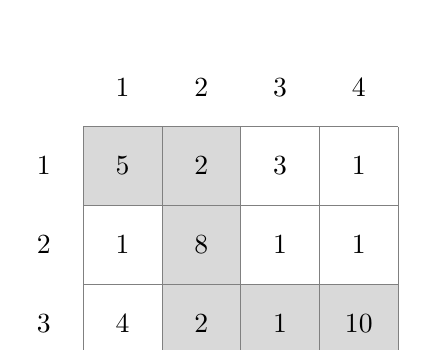
\begin{tikzpicture}
        \fill[gray!30] (0,2) rectangle (1,3);
        \fill[gray!30] (1,2) rectangle (2,3);
        \fill[gray!30] (1,1) rectangle (2,2);
        \fill[gray!30] (1,0) rectangle (2,1);
        \fill[gray!30] (2,0) rectangle (3,1);
        \fill[gray!30] (3,0) rectangle (4,1);

        \draw[gray,very thin] (0,0) grid (4, 3);

        \node at (0.5, 2.5) {5};
        \node at (1.5, 2.5) {2};
        \node at (2.5, 2.5) {3};
        \node at (3.5, 2.5) {1};

        \node at (0.5, 1.5) {1};
        \node at (1.5, 1.5) {8};
        \node at (2.5, 1.5) {1};
        \node at (3.5, 1.5) {1};

        \node at (0.5, 0.5) {4};
        \node at (1.5, 0.5) {2};
        \node at (2.5, 0.5) {1};
        \node at (3.5, 0.5) {10};

        \node at (1.5, 3.5) {2};
        \node at (0.5, 3.5) {1};
        \node at (2.5, 3.5) {3};
        \node at (3.5, 3.5) {4};

        \node at (-0.5, 2.5) {1};
        \node at (-0.5, 1.5) {2};
        \node at (-0.5, 0.5) {3};
    \end{tikzpicture}
    \caption{Exemplo da entrada com células coloridas}
\end{figure}

\vspace{0.3cm}
\textbf{Entrada}

A primeira linha contém dois inteiros $N$ e $M$ ($1 \leq N, M \leq 2000$), representando respectivamente o número de linhas e colunas da grade.

Em seguida, seguem $N$ linhas, cada uma contendo $M$ inteiros $C_{i,j}$ ($0 \leq C_{i,j} \leq 10^4$), representando a quantidade de abóboras em cada posição $i$ e $j$.

\vspace{0.3cm}
\textbf{Saída}

Imprima um único inteiro, sendo o número máximo de abóboras que podem ser colhidas seguindo as regras.

\begin{table}[ht]
    \centering
    \begin{tabular}{|p{7cm}|p{7cm}|}
        \hline
        \begin{center}
            \vspace{-0.3cm}
            \textbf{Exemplos de Entrada}
            \vspace{-0.3cm}
        \end{center} 
         &  
        \begin{center}
            \vspace{-0.3cm}
            \textbf{Exemplos de Saída}
            \vspace{-0.3cm}
        \end{center} \\ \hline
         \texttt{3 4} & \texttt{28} \\
         \texttt{5 2 3 1} & \texttt{} \\
         \texttt{1 8 1 1} & \texttt{} \\
         \texttt{4 2 1 10} & \texttt{} \\
         \hline
    \end{tabular}
    
    \caption{Exemplos de entradas e saídas}
    \label{tab:inputA1}
    
\end{table}

\vspace{0.3cm}

\newpage

\begin{center}
\noindent
\lstinputlisting{abobora_25/A/A5.cpp}
\end{center}
\begin{center}
Problema B

O Desafio do Chocolate do Zé do Grafo

{\small Nome do arquivo: B.c, B.cpp, B.java, ou B.py}

{\large Timelimit: $1$}

{\tiny Por André da Cunha Ribeiro}

\end{center}					

Todo competidor de maratona de programação sabe que as longas horas de um concurso exigem um combustível especial para o cérebro. E qual é o lanche preferido de 10 entre 10 programadores para manter o foco e a energia? Chocolate, é claro! A combinação de açúcar e cafeína parece ter sido feita sob medida para transformar um bug teimoso em um cobiçado "Accepted".

%Zé do Grafo, mais do que um professor, é um mentor que entende perfeitamente a rotina de seus alunos. Vendo sua equipe exausta após um treino intenso para a grande final da competição, ele aparece com o suprimento de energia definitivo: uma enorme barra de chocolate retangular, com N fileiras e M colunas.

%Mas, fiel ao seu estilo, Zé do Grafo não perderia a chance de um bom desafio. Ele colocou a barra de chocolate sobre a mesa e continuou: "O processo para dividir nosso prêmio é simples. A cada movimento, só podemos pegar um único pedaço de chocolate e quebrá-lo uma única vez, sempre em linha reta, seguindo um dos sulcos que dividem os quadrados. Cada quebra transforma um pedaço em dois. Vamos repetir isso até que toda a barra se transforme nos pequenos quadrados individuais de 1x1."

%Ele fez uma pausa e olhou para a equipe com um olhar astuto. "Agora, a pergunta que vale o primeiro pedaço: qual o número exato de quebras necessárias para completar a tarefa?"


Zé do Grafo, um famoso professor de Teoria dos Grafos e um ávido criador de quebra-cabeças, propôs um desafio para seus alunos. Ele apresentou uma barra de chocolate retangular, dividida em pequenos quadrados por sulcos, formando uma grade de $N$ fileiras e $M$ colunas.

O desafio é o seguinte: para dividir a barra de chocolate em $(N * M)$ quadrados de chocolate individuais, os alunos só podem realizar um tipo de movimento. A cada passo, eles podem pegar um único pedaço de chocolate e quebrá-lo ao longo de um dos sulcos (seja na horizontal ou na vertical), resultando em dois pedaços menores.

Sua tarefa é criar um programa que ajude os alunos do Zé do Grafo a descobrir rapidamente o número total de quebras necessárias para transformar a barra inteira em quadrados individuais.

\vspace{0.3cm}
\textbf{Entrada}
A entrada contém  na primeira linha o valor $1 \leq X \leq 1000$ que representa o número dos casos de teste. Seguido de $X$ leituras dos valores de $N,M$ $(1 \leq N,M \leq 10^9)$ indicando as dimensões dos chocolates. 


\vspace{0.3cm}
\textbf{Saída}
Para cada caso de teste, o programa deve produzir uma linha na saída, contendo um único inteiro que representa o número total de quebras necessárias para dividir o chocolate daquele caso de teste.

{\tiny
\begin{table}[h]
    \centering
    \begin{tabular}{|p{7cm}|p{7cm}|}
        \hline
        \begin{center}
            \vspace{-0.3cm}
            \textbf{Exemplos de Entrada}
            \vspace{-0.3cm}
        \end{center} 
         &  
        \begin{center}
            \vspace{-0.3cm}
            \textbf{Exemplos de Saída}
            \vspace{-0.3cm}
        \end{center} \\ \hline
         \texttt{4} & \texttt{3} \\  
         \texttt{2 2} & \texttt{23} \\
         \texttt{4 6} & \texttt{55} \\
         \texttt{7 8} & \texttt{836} \\
         \texttt{27 31} & \texttt{} \\
        \hline
    \end{tabular}
    \caption{Exemplos de entradas e saídas}
\end{table}}

\newpage

\begin{center}
\noindent
\lstinputlisting{abobora_25/B/B5.cpp}
\end{center}

\begin{center}
Problema C

Otimização de Rotas de Coleta de Solo - Simple Smart Agro

{\small Nome do arquivo: C.c, C.cpp, C.java, ou C.py}

{\large Timelimit: $2$}

{\tiny Por Alexandre da Silva}

\end{center}	

\footnotesize
			
A Simple Smart Agro está desenvolvendo um sistema automatizado para coleta de amostras de solo em uma fazenda. O sistema precisa otimizar as rotas de coleta para maximizar a eficiência do processo. Existem $N$ pontos específicos onde amostras de solo devem ser coletadas. O veículo de coleta parte sempre do depósito localizado na origem $(0, 0)$ e deve retornar ao mesmo ponto após coletar todas as amostras. Devido às características do terreno e dos equipamentos, o veículo só pode se mover nas direções cardeais (norte, sul, leste, oeste) e sempre em linha reta entre dois pontos consecutivos da rota. A distância entre dois pontos $(x_1, y_1)$ e $(x_2, y_2)$ é calculada usando a distância Manhattan: $|x_1 - x_2| + |y_1 - y_2|$.

\subsection*{Entrada}

\begin{itemize}
    \item A primeira linha contém um inteiro $N$ $(1 \leq N \leq 10)$, representando o número de pontos de coleta;
    \item As próximas $N$ linhas contêm dois inteiros $x_i$ e $y_i$ $(-1000 \leq x_i, y_i \leq 1000)$, representando as coordenadas do $i$-ésimo ponto de coleta;
       \item Todos os pontos de coleta são distintos entre si;
    \item Nenhum ponto de coleta coincide com a origem $(0,0)$.
\end{itemize}

\subsection*{Saída}

\begin{itemize}
    \item Uma única linha contendo um inteiro: a menor distância total (distância Manhattan) necessária para visitar todos os pontos de coleta e retornar à origem.
\end{itemize}

\subsection*{Exemplos}

\begin{center}
\begin{tabular}{|p{6cm}|p{4cm}|}
\hline
\textbf{Exemplo de Entrada} & \textbf{Exemplo de Saída} \\
\hline
\texttt{3} & \texttt{26} \\
\texttt{2 3} & \\
\texttt{7 1} & \\
\texttt{5 6} & \\
\hline
\texttt{4} & \texttt{42} \\
\texttt{3 4} & \\
\texttt{8 2} & \\
\texttt{12 8} & \\
\texttt{6 10} & \\
\hline
\texttt{1} & \texttt{8} \\
\texttt{2 2} & \\
\hline
\end{tabular}
\end{center}

\subsection*{Explicação do Primeiro Exemplo}

Partindo da origem $(0,0)$, temos os pontos de coleta em $(2,3)$, $(7,1)$ e $(5,6)$.
Uma rota ótima seria:
$(0,0) \rightarrow (2,3) \rightarrow (5,6) \rightarrow (7,1) \rightarrow (0,0)$

Calculando as distâncias:
\begin{itemize}
    \item $(0,0)$ para $(2,3)$: $|2-0| + |3-0| = 2 + 3 = 5$
    \item $(2,3)$ para $(5,6)$: $|5-2| + |6-3| = 3 + 3 = 6$
    \item $(5,6)$ para $(7,1)$: $|7-5| + |1-6| = 2 + 5 = 7$
    \item $(7,1)$ para $(0,0)$: $|0-7| + |0-1| = 7 + 1 = 8$
\end{itemize}

Distância total: $5 + 6 + 7 + 8 = 26$


\newpage

\begin{center}
\noindent
\lstinputlisting{abobora_25/C/C5.cpp}
\end{center}
\begin{center}
Problema D

Agência de Espionagem

{\small Nome do arquivo: D.c, D.cpp, D.java, ou D.py}

{\large Timelimit: $1$}

{\tiny Por Athos José}


\end{center}

A Agência Nacional de Espionagem mantém em seus cofres uma coleção de símbolos secretos, representados por uma sequência de letras. Esses símbolos podem ser reorganizados em qualquer ordem, de forma a formar novas mensagens.

Agentes inimigos, porém, estão tentando criar mensagens escondidas dentro dessas reorganizações. Uma mensagem inimiga é considerada possível se puder aparecer como uma sequência contínua de caracteres de alguma permutação dos símbolos guardados no cofre.

Sua missão é, para cada mensagem inimiga recebida, determinar se ela pode ser formada a partir dos símbolos da Agência.

\vspace{0.3cm}
\textbf{Entrada}

A primeira linha contém um inteiro $N$ ($1 \leq N \leq 10^5$), o número de mensagens inimigas a serem analisadas, seguido de uma string $S$ ($1 \leq |S| \leq 10^5$) representando os símbolos secretos do cofre.

Cada uma das próximas $N$ linhas contém uma string $Q_i$ ($1 \leq |Q_i| \leq 10^5$), representando uma mensagem inimiga a ser verificada.

A soma dos comprimentos de todas as mensagens $Q_i$ não excede $10^9$.

Todas as strings são compostas apenas de letras minúsculas do alfabeto inglês (a-z).

\vspace{0.3cm}
\textbf{Saída}

Para cada mensagem $Q_i$ imprima uma linha contendo:
\begin{itemize}
    \item ``SIM'', se a mensagem pode ser formada como substring de alguma permutação de $S$.
    \item ``NAO'',caso contrário.
\end{itemize}

\begin{table}[h]
    \centering
    \begin{tabular}{|p{7cm}|p{7cm}|}
       \hline
        \begin{center}
            \vspace{-0.3cm}
            \textbf{Exemplos de Entrada}
            \vspace{-0.3cm}
        \end{center} 
         &  
        \begin{center}
            \vspace{-0.3cm}
            \textbf{Exemplos de Saída}
            \vspace{-0.3cm}
        \end{center} \\ \hline
         \texttt{3 abac} & \texttt{SIM} \\  
         \texttt{caa} & \texttt{NAO} \\
         \texttt{aaa} & \texttt{SIM} \\  
         \texttt{bac} & \\
         \hline
    \end{tabular}
    \caption{Exemplos de entradas e saídas}
    \label{tab:inputB}
\end{table}

\newpage

\begin{center}
\noindent
\lstinputlisting{abobora_25/D/D5.cpp}
\end{center}
\begin{center}
Problema E

Estória da Estônia

{\small Nome do arquivo: E.c, E.cpp, E.java, ou E.py}

{\large Timelimit: $1$}

{\tiny Por Márcio Belo}

\end{center}			

O professor Márcio Belo sempre gostou de charadas matemáticas. Um dia ele se deparou com uma estória, pra lá da Estônia. Dado um número primo ímpar $p$, sempre é possível um triângulo de lados inteiros $x$, $y$ e $z$, em ordem crescente de tamanho com as seguintes propriedades: 
\begin{itemize}
    \item A diferença da soma dos lados menores do triângulo pelo lado maior é igual ao primo $p$; 
    \item A diferença da soma das áreas dos quadrados de lados $x$ e $y$ e a área do quadrado de lado $z$ é igual ao primo $p$. 
\end{itemize}
Em matematiquês:

\vspace{3mm}
Dado um primo $p \geq 3$, sempre existem triplas $(x,y,z)$, com $x \leq y \leq z$ que satisfazem: 
\begin{align*}
    x + y - z & = p \\
    x^{2} + y^{2} - z^{2} & = p 
\end{align*}
Quem são essas triplas $(x,y,z)$? Você pode ajudar o professor?

\vspace{0.3cm}
\textbf{Entrada}
Cada entrada contém uma única linha com o número primo $p$, com $(3 \leq p < 2^{16})$. 

\vspace{0.3cm}
\textbf{Saída}
O sistema deve retornar todas as triplas $(x,y,z)$ em ordem crescente de $x$. Uma tripla por linha,  

\begin{table}[h]
    \centering
    \begin{tabular}{|p{7cm}|p{7cm}|}
        \hline
        \begin{center}
            \vspace{-0.3cm}
            \textbf{Exemplos de Entrada}
            \vspace{-0.3cm}
        \end{center} 
         &  
        \begin{center}
            \vspace{-0.3cm}
            \textbf{Exemplos de Saída}
            \vspace{-0.3cm}
        \end{center} \\ \hline
         \texttt{3} & \texttt{(4,6,7)} \\  
         \hline
         \texttt{5} & \texttt{(6, 15, 16)} \\ 
          & \texttt{(7, 10, 12)} \\ 
         \hline
         \texttt{13} & \texttt{(14, 91, 92)} \\
         & \texttt{(15, 52, 54)} \\
         & \texttt{(16, 39, 42)} \\
         & \texttt{(19, 26, 32)} \\ 
         \hline
         \texttt{65267} & \texttt{(65268,2129923278,2129923279)} \\ 
          & \texttt{(97900,130534,163167)} \\ 
         \hline
    \end{tabular}
    \caption{Exemplos de entradas e saídas}

\end{table}

\newpage
\begin{center}
\noindent
\lstinputlisting{abobora_25/E/E5.cpp}
\end{center}
\begin{center}
Problema F

Monitorando Pragas

{\small Nome do arquivo: F.c, F.cpp, F.java, ou F.py}

{\large Timelimit: $1$}

{\tiny Por Emanuel Silva Araujo}

\end{center}

\footnotesize

O agricultor Seu Jayme sofre constantemente com infestações de insetos em sua lavoura de soja. Para reduzir perdas e otimizar o manejo, ele procurou a EMBRAPII para desenvolver uma ferramenta de monitoramento diário de pragas.
Sua tarefa como programador é implementar um programa que leia os valores de população diária e identifique situações de risco, emitindo alertas de acordo com os seguintes critérios:
%Critérios de Alerta
    \begin{itemize}
        \item  Alerta por pico diário [Pico]
        \begin{itemize}
            \item Se em qualquer dia a população registrada ultrapassar 200 insetos.
        \end{itemize}
        \item  Alerta por variação em 7 dias [7 Dias]
        \begin{itemize}
            \item Se a diferença percentual entre o valor mínimo e o máximo em um intervalo de 7 dias consecutivos for maior ou igual a 20\%.
        \end{itemize}
        \item  Alerta por crescimento contínuo [Crescimento]
        \begin{itemize}
            \item Se ocorrerem 4 dias seguidos de crescimento, e em cada dia a população for pelo menos 5\% maior que a do dia anterior.
        \end{itemize}
    \end{itemize}
        
\vspace{0.3cm}
\textbf{Entrada}

Um número inteiro $(0 <= N <= 360)$, representando a quantidade de dias monitorados (entre os dias $0$ e $360$).
Uma sequência de $N$ números inteiros $(0 < X <= 5000)$, cada um representando a estimativa da população de insetos no respectivo dia.

\vspace{0.3cm}
\textbf{Saída}

    Para cada alerta identificado, o programa deve imprimir:
    \begin{itemize}
        \item O tipo do alerta;
        \item O(s) dia(s) correspondente(s);
        \item O valor percentual (quando aplicável), com duas casas decimais.
    \end{itemize}
    Caso não tenha nenhum alerta, deve imprimir uma mensagem de "Nenhum Alerta".
    Para dias que tiveram mais de um alerta a ordem de impressão é: $[Pico] > [7 Dias] > [Crescimento]$.
 
\begin{table}[h]
    \centering
    \footnotesize
    \begin{tabular}{|p{8cm}|p{8cm}|}
        \hline
        \begin{center}
            \vspace{-0.3cm}
            \textbf{Exemplos de Entrada}
            \vspace{-0.3cm}
        \end{center} 
         &  
        \begin{center}
            \vspace{-0.3cm}
            \textbf{Exemplos de Saída}
            \vspace{-0.3cm}
        \end{center} \\ \hline
		    \texttt{10} & \texttt{[Crescimento] 1-4: maior que >= 5\% } \\
                \texttt{50 60 70 80 90 200 210 220 180 170} & \texttt{[Crescimento] 1-5: maior que >= 5\% } \\
& \texttt{[Crescimento] 1-6: maior que >= 5\% } \\
& \texttt{[Pico] 7: 210 insetos} \\
& \texttt{[7 Dias] 1-7: 320.00\%} \\
& \texttt{[Crescimento] 1-7: maior que >= 5\% } \\
& \texttt{[Pico] 8: 220 insetos} \\
& \texttt{[7 Dias] 2-8: 266.67\%} \\
& \texttt{[7 Dias] 3-9: 214.29\%} \\
& \texttt{[7 Dias] 4-10: 175.00\%} \\


         \hline
   		    \texttt{9}   & \texttt{[Crescimento] 1-4: maior que >= 5\% } \\
            \texttt{100 105 112 118 90 96 100 120 80} & \texttt{[7 Dias] 2-8: 33.33\%} \\
         \hline    
   		    \texttt{8}   & \texttt{Nenhum Alerta} \\
            \texttt{118 120 118 140 140 140 130 100} & \\
         \hline    
    \end{tabular}
    \caption{Exemplos de entradas e saídas}

\end{table}

\normalsize

\newpage

\begin{center}
\lstinputlisting{abobora_25/F/F5.cpp}
\end{center}

\begin{center}
Problema G

Comportamento Dinâmico

{\small Nome do arquivo: G.c, G.cpp, G.java, ou G.py}

{\large Timelimit: $1$}

{\tiny Por Heverton Barros de Macêdo}

\end{center}

\footnotesize

	Durante uma investigação sobre o comportamento de sistemas dinâmicos, Wolfram definiu o seguinte cenário para efetuar experimentos: dada uma cadeia de $N$ células, linearmente distribuídas, cada célula armazena um único estado (bit), e além disso as células das extremidades são vizinhas entre si. Para cada instante de tempo $t$ a evolução dessa cadeia ocorre simultaneamente em todas as células, considerando uma regra de evolução previamente definida. Essa regra é aplicada a cada vizinhança de $K=3$ células gerando um novo estado, conforme indicado na Tabela~\ref{tab:evolucao}.
	
	\begin{table}[h!]
		\caption{Regra aplicada para evolução do experimento de Wolfram.}
		\label{tab:evolucao}
		
		\centering
		\footnotesize{
		\begin{tabular}{|c|c|c|c|c|c|c|c|c|}
			\hline
			\cellcolor[HTML]{DDDDDD} Regra para vizinhança & 000 & 001 & \cellcolor[HTML]{FFAAAA} 010 & 011 & 100 & 101 & 110 & 111 \\ \hline
			\cellcolor[HTML]{DDDDDD} Novo estado para célula central & 1 & 0 &  \cellcolor[HTML]{AAFFAA} 0 & 1 & 0 & 0 & 0 & 1 \\ \hline
		\end{tabular}
		}
	\end{table}

Como exemplo, considere um experimento (veja a Tabela~\ref{tab:exemplo_evolucao}) com a cadeia de bits formada por $11$ células ($N = 11$), em que no instante $t = 0$ apenas um bit, exatamente no centro da cadeia, possui o estado $1$ e as demais células possuem o estado $0$, evoluindo por $4$ passos de tempo ($t = 4$).
%Como exemplo, considere um experimento (veja a Tabela~\ref{tab:exemplo_evolucao}) com a cadeia de bits no espaço linear formada por $11$ células ($N = 11$), em que apenas um bit, exatamente no centro da cadeia ($t = 0$), possui o estado $1$ e as demais células possuem o estado $0$, evoluindo por $4$ passos de tempo.

A Tabela~\ref{tab:exemplo_evolucao} ilustra o experimento com a configuração inicial ($t = 0$) formada por: $00000100000$. No próximo passo de tempo ($t = 1$), todas as células evoluem (podem alterar o estado) considerando a vizinhança indicada na regra (Tabela~\ref{tab:evolucao}). Em destaque na cor vermelha (Tabelas~\ref{tab:evolucao} e ~\ref{tab:exemplo_evolucao}) está a atualização da célula central, formada pela vizinhança $010$ que, segundo a regra, deve evoluir no próximo passo de tempo ($t = 1$) para o estado $0$ (destaque na cor verde). É possível notar no exemplo, a evolução da cadeia inicial por $4$ passos de tempo. Vale destacar que as células na extremidade (esquerda e direta) estão conectadas (formato de anel - toroidal)

	\begin{table}[h!]
	\caption{Exemplo de um experimento por $4$ passos de tempo.}
	\label{tab:exemplo_evolucao}
	
	\centering
	\footnotesize{	
	\begin{tabular}{|c|c|c|c|c|c|c|c|c|c|c|c|}
		\hline
		Tempo & \multicolumn{11}{c|}{Cadeia linear de N células}\\ \hline
    	$t = 0$ & 0 & 0 & 0 & 0 & \cellcolor[HTML]{FFAAAA} 0 & \cellcolor[HTML]{FFAAAA} 1 & \cellcolor[HTML]{FFAAAA} 0 & 0 & 0 & 0 & 0 \\ \hline
		$t = 1$ & 1 & 1 & 1 & 1 &  0 & \cellcolor[HTML]{AAFFAA} 0 & 0 & 1 & 1 & 1 & 1 \\ \hline
		$t = 2$ & 1 & 1 & 1 & 0 &  1 & 0 & 0 & 1 & 1 & 1 & 1 \\ \hline
		$t = 3$ & 1 & 1 & 0 & 0 &  0 & 0 & 0 & 1 & 1 & 1 & 1 \\ \hline
		$t = 4$ & 1 & 0 & 0 & 1 &  1 & 1 & 0 & 1 & 1 & 1 & 1 \\ \hline
	\end{tabular}
	}	
\end{table}

%\pagebreak
Sua missão é ajudar Wolfram a obter a configuração dos estados após $t$ passos de tempo, considerando uma
sequência inicial qualquer no tempo $t = 0$ e a aplicação da regra indicada no enunciado.

\vspace{0.3cm}
\textbf{Entrada}

A entrada contém vários casos de teste. Cada linha contém um inteiro $t$ ($0~<~t~\leq~1000$), que representa
a quantidade de passos de evolução, seguido pela cadeia de bits no tempo $t = 0$, que pode variar conforme a
quantidade de células da amostra $N$ ($3 \leq N < 100$).

\vspace{0.3cm}
\textbf{Saída}

O programa deve produzir como saída a configuração da cadeia no espaço linear de células após a evolução
de $t$ passos de tempo.

\begin{table}[h]
    \centering
    \footnotesize
    \begin{tabular}{|p{8cm}|p{8cm}|}
        \hline
        \begin{center}
            \vspace{-0.3cm}
            \textbf{Exemplos de Entrada}
            \vspace{-0.3cm}
        \end{center} 
         &  
        \begin{center}
            \vspace{-0.3cm}
            \textbf{Exemplos de Saída}
            \vspace{-0.3cm}
        \end{center} \\ \hline
		    \texttt{1 00000100000} & \texttt{11110001111} \\
         \hline
   		    \texttt{2 00000100000} & \texttt{11100101111} \\
         \hline    
   		    \texttt{3 00000100000} & \texttt{11000001111} \\
         \hline    
   		    \texttt{578 00000100000} & \texttt{00000111101} \\
         \hline    
   		    \texttt{978 011001111000110111010011} & \texttt{100111000001110000011101} \\
         \hline    
    \end{tabular}
    \caption{Exemplos de entradas e saídas}    
\end{table}

\normalsize

\newpage

\begin{center}
\noindent
\lstinputlisting{abobora_25/G/G5.cpp}
\end{center}
\bibliography{references}

\end{document}